\documentclass{beamer}

\usepackage{graphicx}
\usepackage{bm}
\usepackage{tabularx}
\usepackage{textcomp}
\usepackage{multirow}
\usepackage{mathtools}
%\usepackage{epstopdf}

% Import the UNCMath theme.
% UNC is the default color theme.
\usetheme{UNCMath}

% Uncomment to use a different color scheme.
%\definecolor{darkpurple}{rgb}{0.2,0,0.2}
%\setbeamercolor*{structure}{fg=black,bg=darkpurple}

\logo{

\includegraphics[height=3em]{oldwell_cmyk}
}

% A macro for making the title frame.
% Removes the bottom bar and logo temporarily.
% If you don't want these in other frames, 
% you could try mimicking this.
\newcommand{\titleframe}{
{
\setbeamertemplate{headline}{}
\setbeamertemplate{footline}{}
\begin{frame}
\titlepage
\end{frame}
}
}

\newcommand{\mB}{\textbf{B}}
\newcommand{\mQ}{\textbf{Q}}
\newcommand{\mR}{\textbf{R}}
\newcommand{\mP}{\textbf{P}}
\newcommand{\mX}{\textbf{X}}
\newcommand{\mY}{\textbf{Y}}
\newcommand{\mx}{\textbf{x}}
\newcommand{\my}{\textbf{y}}
\newcommand{\mM}{\textbf{M}}
\newcommand{\mH}{\textbf{H}}
\newcommand{\mK}{\textbf{K}}
\newcommand{\mI}{\textbf{I}}

\newcommand{\meps}{\bm{\epsilon}}
\newcommand{\meta}{\bm{\eta}}

\newcommand{\vx}{\bm{x}}
\newcommand{\vw}{\bm{w}}
\newcommand{\vW}{\bm{W}}

\newcommand{\vb}{\bm{b}}
\newcommand{\vy}{\bm{y}}


\newcommand{\cN}{\mathcal{N}}
\newcommand{\cH}{\mathcal{H}}
\newcommand{\cM}{\mathcal{M}}

%%%%%%%%%%%%%%%%%%%%%%%%%%%%%%%%%%%%%%%%%%
%
% Information for the title frame.
%
\title{Data Assimilation with\\ Machine Learning Observation Operator}
\subtitle{an Application on Melt Pond Problem}
\author[Siyang Jing]{Siyang Jing}
\institute{Department of Mathematics, University of North Carolina at Chapel Hill}
\date{March 28th, 2019}

%%%%%%%%%%%%%%%%%%%%%%%%%%%%%%%%%%%%%%%%%%
%
% Start of document.
%
\begin{document}

% This is the titleframe, do it this way 
% so that you don't have the logo on the title page.
\titleframe


\begin{frame}
\frametitle{Introduction to Data Assimilation}
\centering
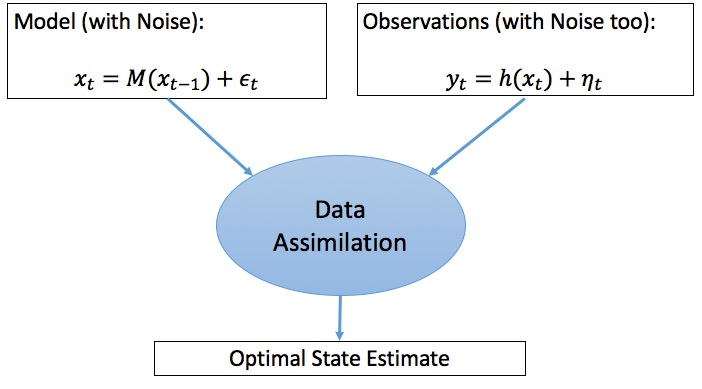
\includegraphics[width=0.6\linewidth]{Figures/DAIntro.jpeg}
\begin{itemize}
\item Mathematical model is never a perfect description of the real world, e.g. dynamical systems from physical laws.
\item Measurements, or observations, always come with error or uncertainty.
\item Data assimilation is a way to combine these two types of information.
\end{itemize}
\end{frame}

\begin{frame}
\frametitle{Introduction to Data Assimilation}
\begin{columns}
\begin{column}{0.4\textwidth}
	\begin{enumerate}
		\item Prediction step: $\mx_{t+1}^f=\cM(\mx_t^a)$ \\ 
				$\mx^f$: the forecast
		\item Update step: $\mx^a=\mx^f + \mK(\my - \cH(\mx^f))$\\ $\mK$: Kalman gain matrix \\
				$\mx^a$: the analysis
		\item Repeat the steps.
	\end{enumerate}
\end{column}
\begin{column}{0.6\textwidth} 
    \begin{center}
    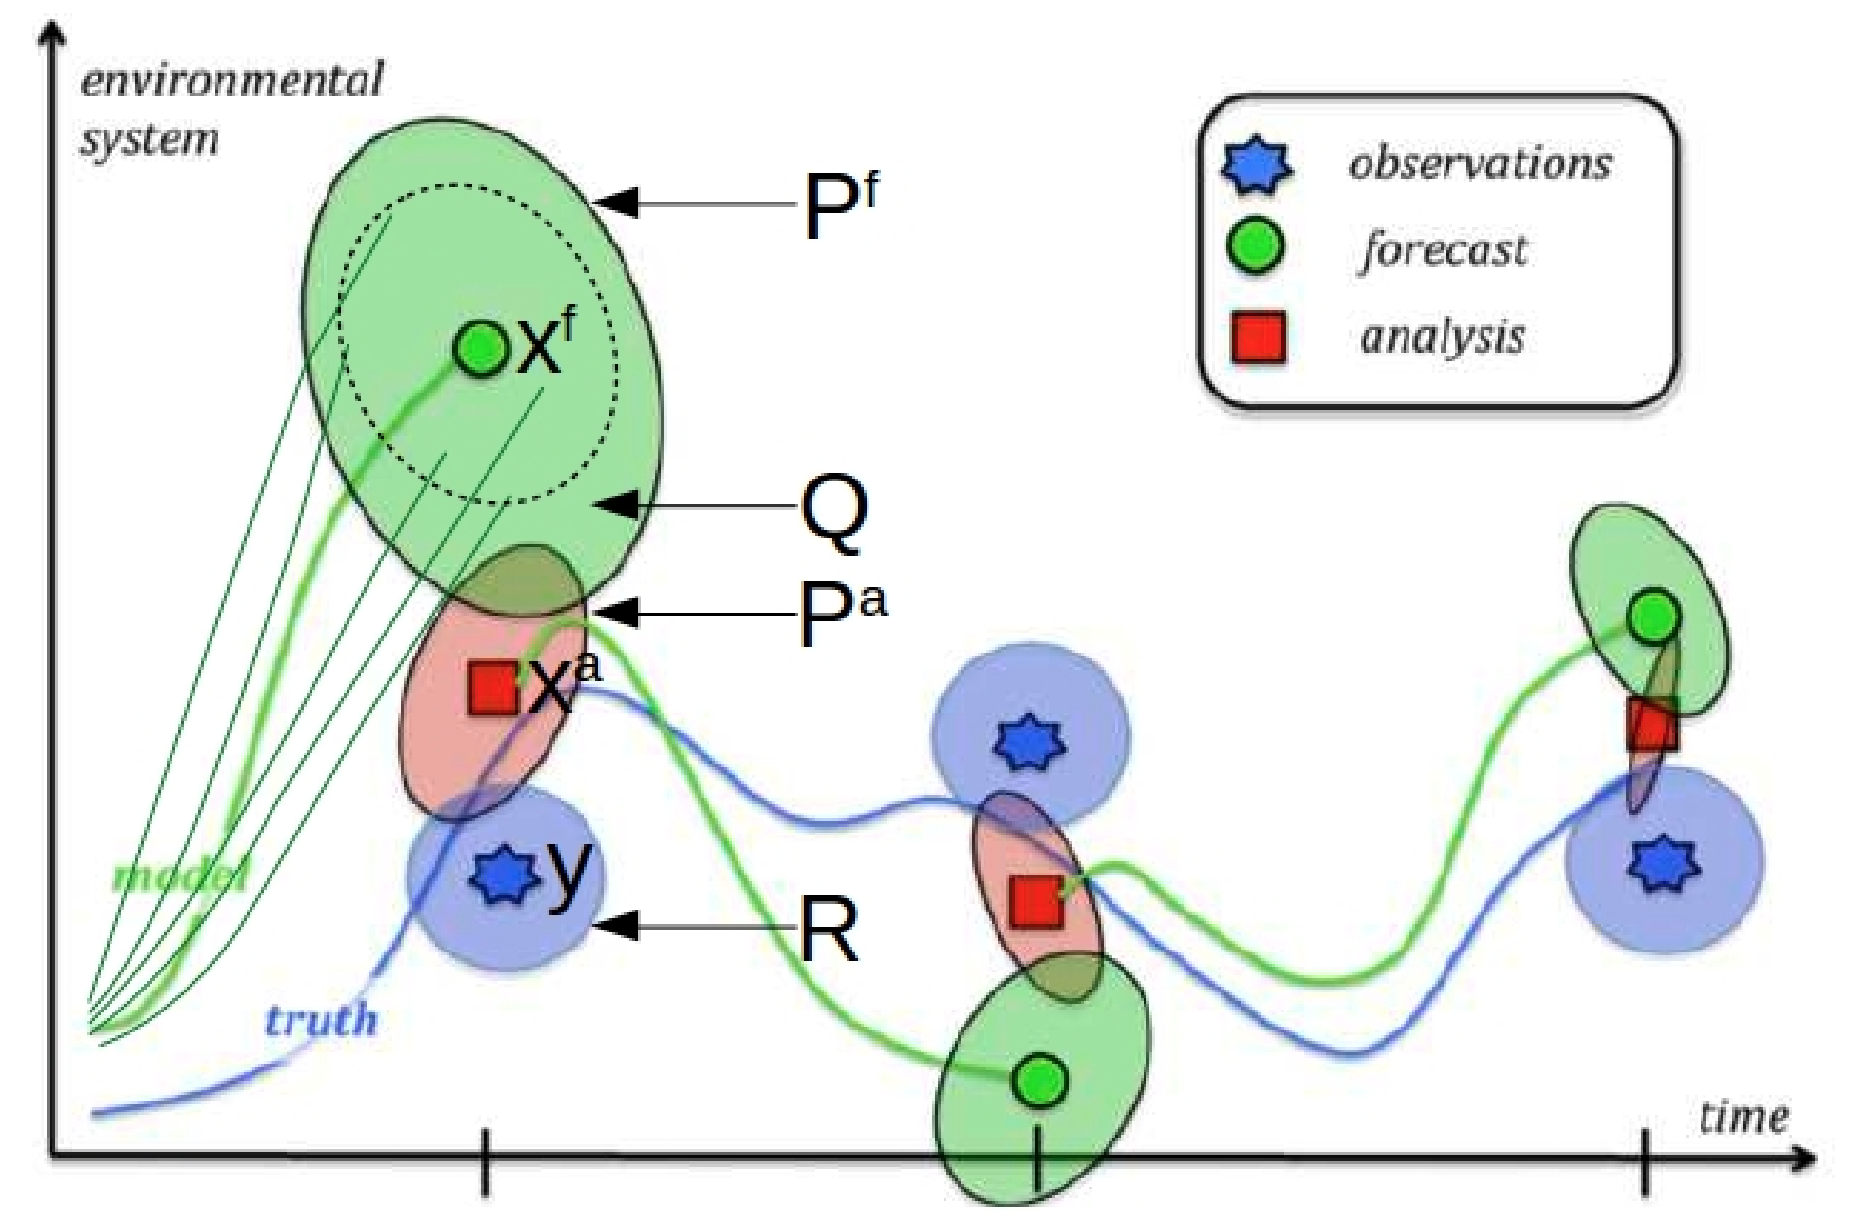
\includegraphics[width=\linewidth]{Figures/DAVisualization.png}
    \end{center}
\end{column}
\end{columns}
\end{frame}

\begin{frame}
\frametitle{Ensemble Kalman Filter}
\begin{center}
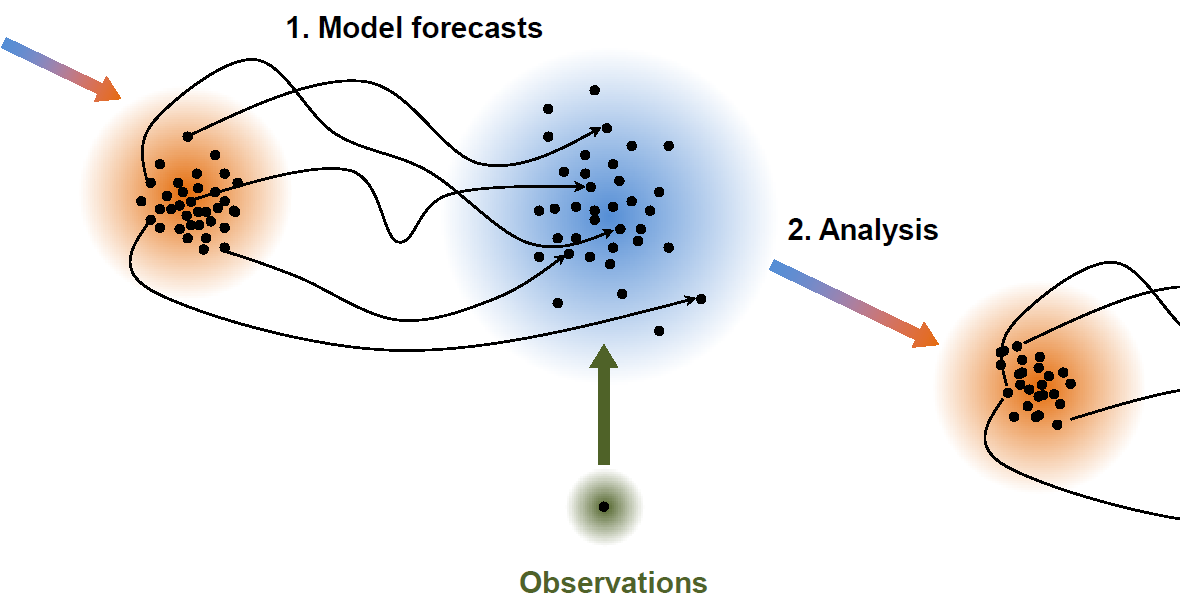
\includegraphics[width=0.6\linewidth]{Figures/EnKF.png}
\end{center}

\begin{enumerate}
\item Ensemble members from last step
\item Evolve under model
\item Covariance matrix $\mP$ from ensemble
\item Update ensemble using Kalman filter with $\mK$ based on covariance $\mP$
\item New ensemble for the next step
\end{enumerate}
\end{frame}

\begin{frame}
\frametitle{Sea Ice Concentration}
\begin{itemize}
	\item The polar regions are typically cloudy restricting continuous sea ice observations in the visible spectrum.
	\item Microwaves pass right through the clouds and microwave radiometry can provide continuous daily observations of sea ice concentration.
	\item NASA has an algorithm to retrieve ice concentration from satellite radiance.
\end{itemize}
\end{frame}

\begin{frame}
\frametitle{Problem with Melt Ponds}
\centering
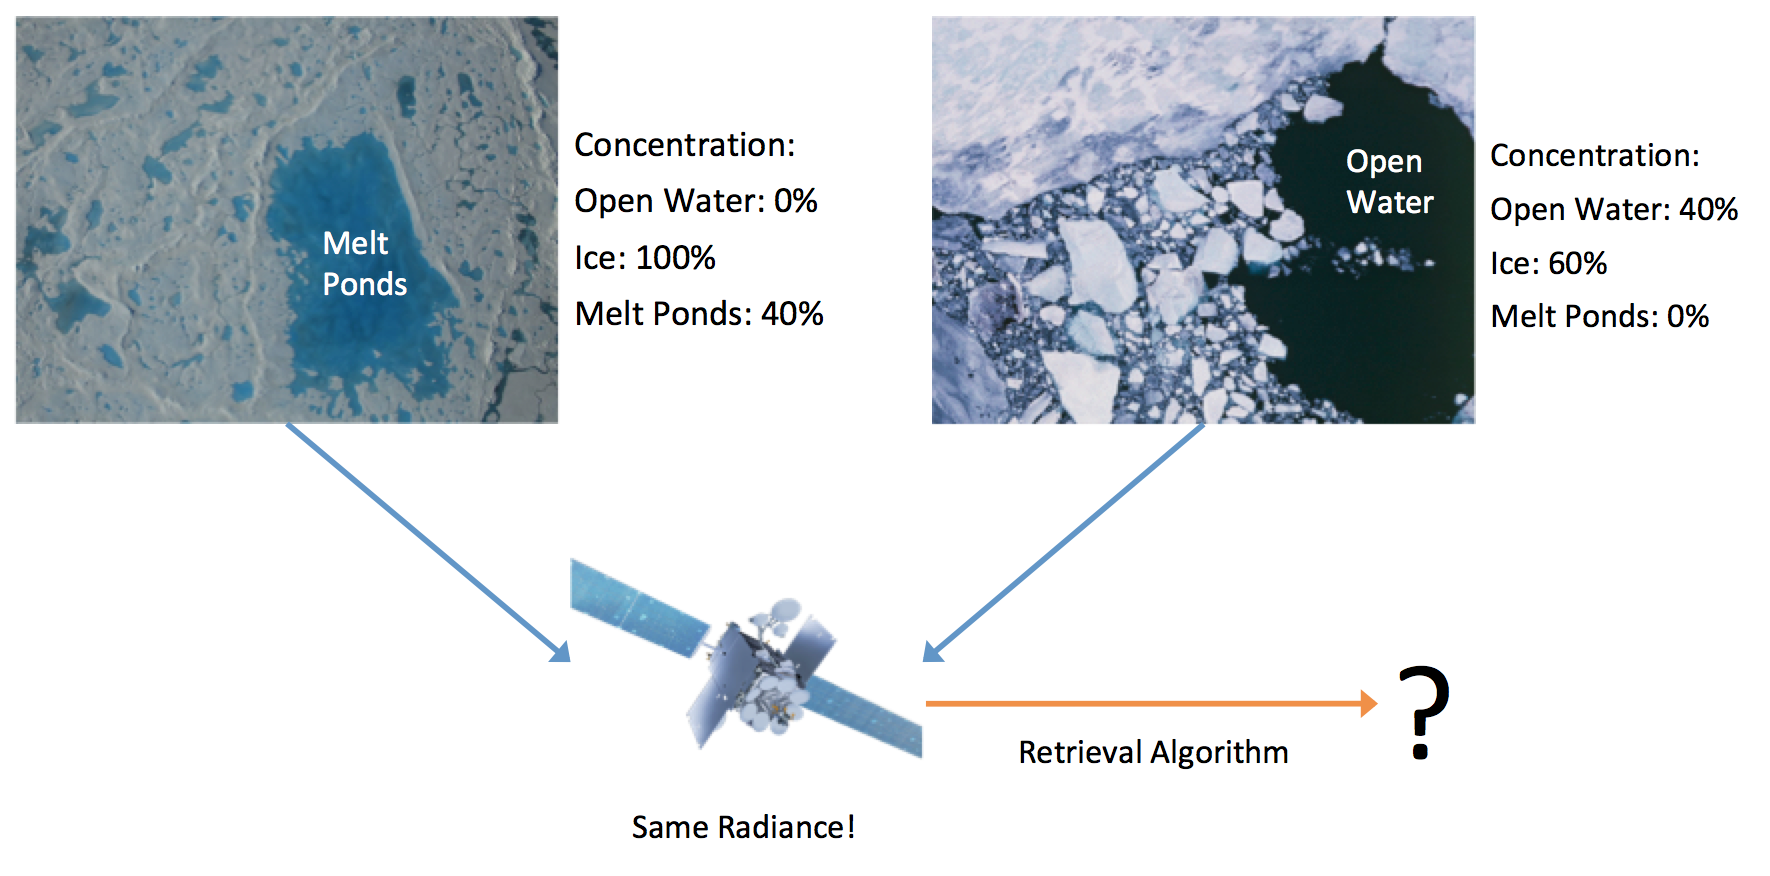
\includegraphics[width=0.8\linewidth]{Figures/MeltPondsProblem.png}
\begin{itemize}
	\item Melt ponds have the same microwave signature as open water and obscure the signature of the ice below them. Therefore both the situations look roughly the same to the satellite.
	\item The retrieval algorithm will likely give incorrect ice concentration.
	\item Assimilating on wrong information makes the state estimation worse.
	\item e.g. Models predicts 90\%, but observation is 60\%. More error added!
\end{itemize}

\end{frame}

\begin{frame}
\frametitle{Assimilate with Radiance}
\begin{itemize}
	\item Change the observation space
	\begin{itemize}
		\item Before: states {\textrightarrow} satellite radiance {\textrightarrow} (wrong) concentration
		\item Proposed: states {\textrightarrow} satellite radiance
	\end{itemize}
	\item Challenge: How to get $\cH$: states {\textrightarrow} satellite radiance
	\begin{itemize}
		\item Mathematical atmospheric model requires heavy computation. Not efficient and sometimes not accurate.
		\item With sufficient historic data of sea ice optical images and corresponding satellite radiances, we can use machine learning to construct the observation operator.
	\end{itemize}
	\item To test out our idea and to investigate the potential challenges in this approach, we start with a test bed model and synthetic data.
\end{itemize}
\end{frame}

\begin{frame}
\frametitle{Test Bed Model}
\begin{itemize}
	\item Instead of directly modeling ice concentration and other variables, we model the energy $E$ and maximum attainable albedo $\alpha_m$.
	\item Therefore, the state vector is 
\[\mx =[E\quad \alpha_m]\]
	\item The albedo can be calculated as 
\[\alpha(E,\alpha_m)=\frac{\alpha_{ml}+\alpha_m}{2}+\frac{\alpha_{ml}-\alpha_m}{2}\tanh\left(\frac{E}{L_i h_{c}} \right)\]
\end{itemize}
\end{frame}
\begin{frame}
\frametitle{Test Bed Model: Dynamical System}
{\setlength{\parskip}{0.5em}
\begin{itemize}
\item When the temperature is high, which is corresponding to $\alpha(E,\alpha_m)>0.6$ \par
$\frac{dE}{dt}=[1-\alpha(E,\alpha_{m})]F_s(t)-F_0(t)+F_{co_2}-F_T(t)\frac{E}{c_{ml} H_{ml}}+F_B $ \par
$\frac{d \alpha_{m}}{dt}= \frac{E^2}{K^2}\alpha_{m}\left(1-\frac{\alpha_{m}}{0.8}\right) + \frac{K^2}{1+E^2}\alpha_{m}\left(1-\frac{\alpha_{m}}{0.6}\right) $ \par
\item When the temperature is low, which is corresponding to $\alpha(E,\alpha_m)<0.6$ \par
$\frac{dE}{dt}=[1-\alpha(E,\alpha_{m})]F_s(t)-F_0(t)+F_{co_2}-F_T(t)\frac{E}{c_{ml} H_{ml}}+F_B $\par
$\frac{ d \alpha_{m}}{dt}=\frac{K^2}{1+E^2}\alpha_{m}\left(1-\frac{\alpha_{m}}{0.6}\right) +\frac{E^2}{K^2}\alpha_{m}\left(1-\frac{\alpha_{m}}{0.2}\right)$ \par
\item One of the parameters of particular interest $F_{co_2}$: a combination of all exterior factors that contribute to the heat in the system, mainly the amount of $CO_2$.
\end{itemize}
}
\end{frame}

\begin{frame}
\frametitle{Test Bed Model: Dynamical System}
\centering
\includegraphics[width=\linewidth]{Figures/fc=-10_new.png}
\end{frame}
\begin{frame}
\frametitle{Test Bed Model: Dynamical System}
\centering
\includegraphics[width=\linewidth]{Figures/fc=0_new.png}
\end{frame}
\begin{frame}
\frametitle{Test Bed Model: Dynamical System}
\centering
\includegraphics[width=\linewidth]{Figures/fc=10_new.png}
\end{frame}
\begin{frame}
\frametitle{Test Bed Model: Dynamical System}
\centering
\includegraphics[width=\linewidth]{Figures/fc=20_new.png}
\end{frame}
\begin{frame}
\frametitle{Test Bed Model: Dynamical System}
\centering
\includegraphics[width=\linewidth]{Figures/fc=30_new.png}
\end{frame}
\begin{frame}
\frametitle{Test Bed Model: Dynamical System}
\centering
\includegraphics[width=\linewidth]{Figures/fc=40_new.png}
\end{frame}
\begin{frame}
\frametitle{Test Bed Model: Dynamical System}
\centering
\includegraphics[width=\linewidth]{Figures/fc=50_new.png}
\end{frame}
\begin{frame}
\frametitle{Test Bed Model: Dynamical System}
\centering
\includegraphics[width=\linewidth]{Figures/fc=60_new.png}
\end{frame}
\begin{frame}
\frametitle{Test Bed Model: Dynamical System}
\centering
\includegraphics[width=\linewidth]{Figures/fc=70_new.png}
\end{frame}
\begin{frame}
\frametitle{Test Bed Model: Dynamical System}
\centering
\includegraphics[width=\linewidth]{Figures/fc=80_new.png}
\end{frame}
\begin{frame}
\frametitle{Test Bed Model: Dynamical System}
\centering
\includegraphics[width=\linewidth]{Figures/fc=90_new.png}
\end{frame}
\begin{frame}
\frametitle{Test Bed Model: Dynamical System}
\centering
\includegraphics[width=\linewidth]{Figures/fc=100_new.png}
\end{frame}
\begin{frame}
\frametitle{Test Bed Model: Dynamical System}
The trajectory that we use in data assimilation experiment.
\centering
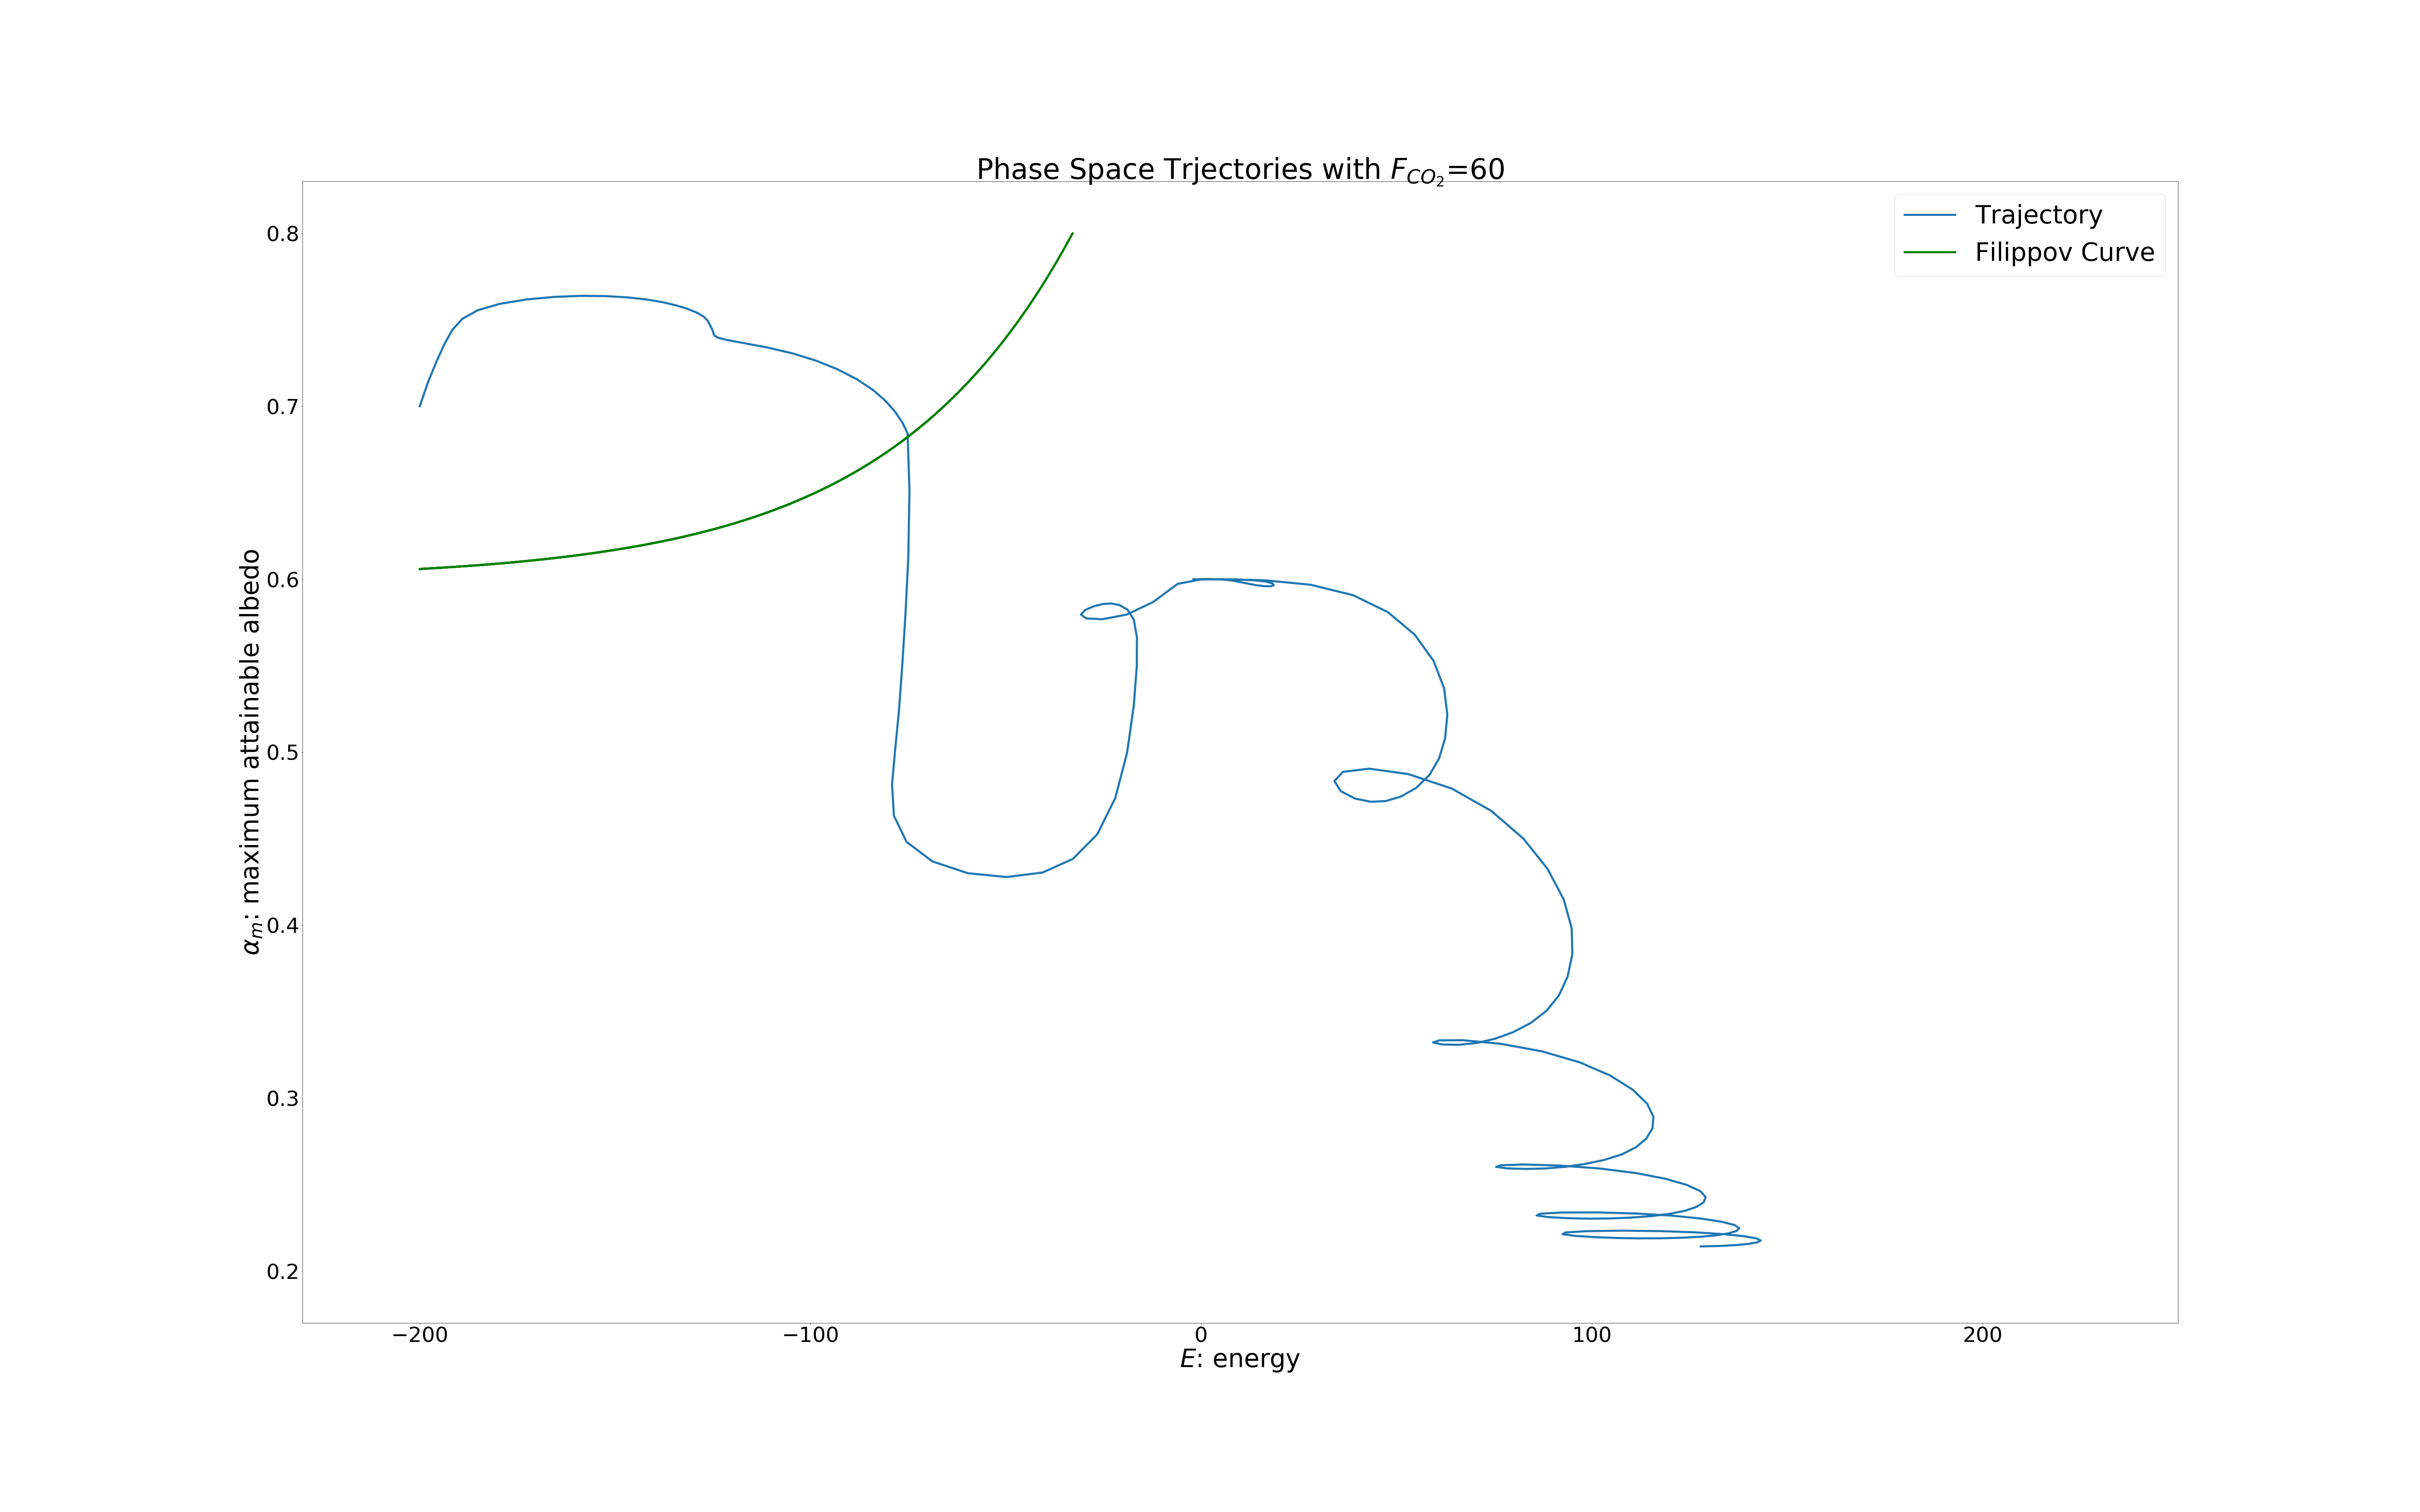
\includegraphics[width=\linewidth]{Figures/fc=60E=-200am=0_7.png}
\end{frame}

\begin{frame}
\frametitle{Test Bed Model: Observations}
\centering
\begin{tabular}{|c|c|}\hline
Ice concentration & $C_i=1-\left(\frac{0.8-\frac{1}{2}\left( \alpha_m+\alpha(E,\alpha_m)\right)}{0.6}\right)$\\ \hline
Pond concentration & $C_p=1-\frac{\alpha(E,\alpha_m)}{\alpha_m}$ \\ \hline
\multirow{5}{*}{Satellite Radiances} 
& $|E\alpha_m|$\\ 
& $\alpha_m-\alpha(E,\alpha_m)$\\
& $\alpha(E,\alpha_m)|E|$\\
& $(0.5+0.4\tanh(\frac{50-E}{10}))(E+273.15)$\\
& $C_i C_p$\\ \hline

Satellite retrieval & \multirow{2}{*}{$C_{sat}=\max(0,C_i-C_p)$}\\
concentration & \\ \hline
\end{tabular}
$C_{sat}$ is supposed to give $C_i$, but instead subtracts $C_p$ from it. If we still assume $C_{sat}$ gives the correct value of $C_i$ and use it in data assimilation, error will be incorporated in the analysis.
\end{frame}

\begin{frame}
\frametitle{Test Bed Model: Observations}
The following figure shows the error in satellite retrieved sea ice concentration.\par
Note that the error is especially large when energy is larger than $0$, corresponding to the situation when temperature rises and melt ponds starts to form.
\begin{center}
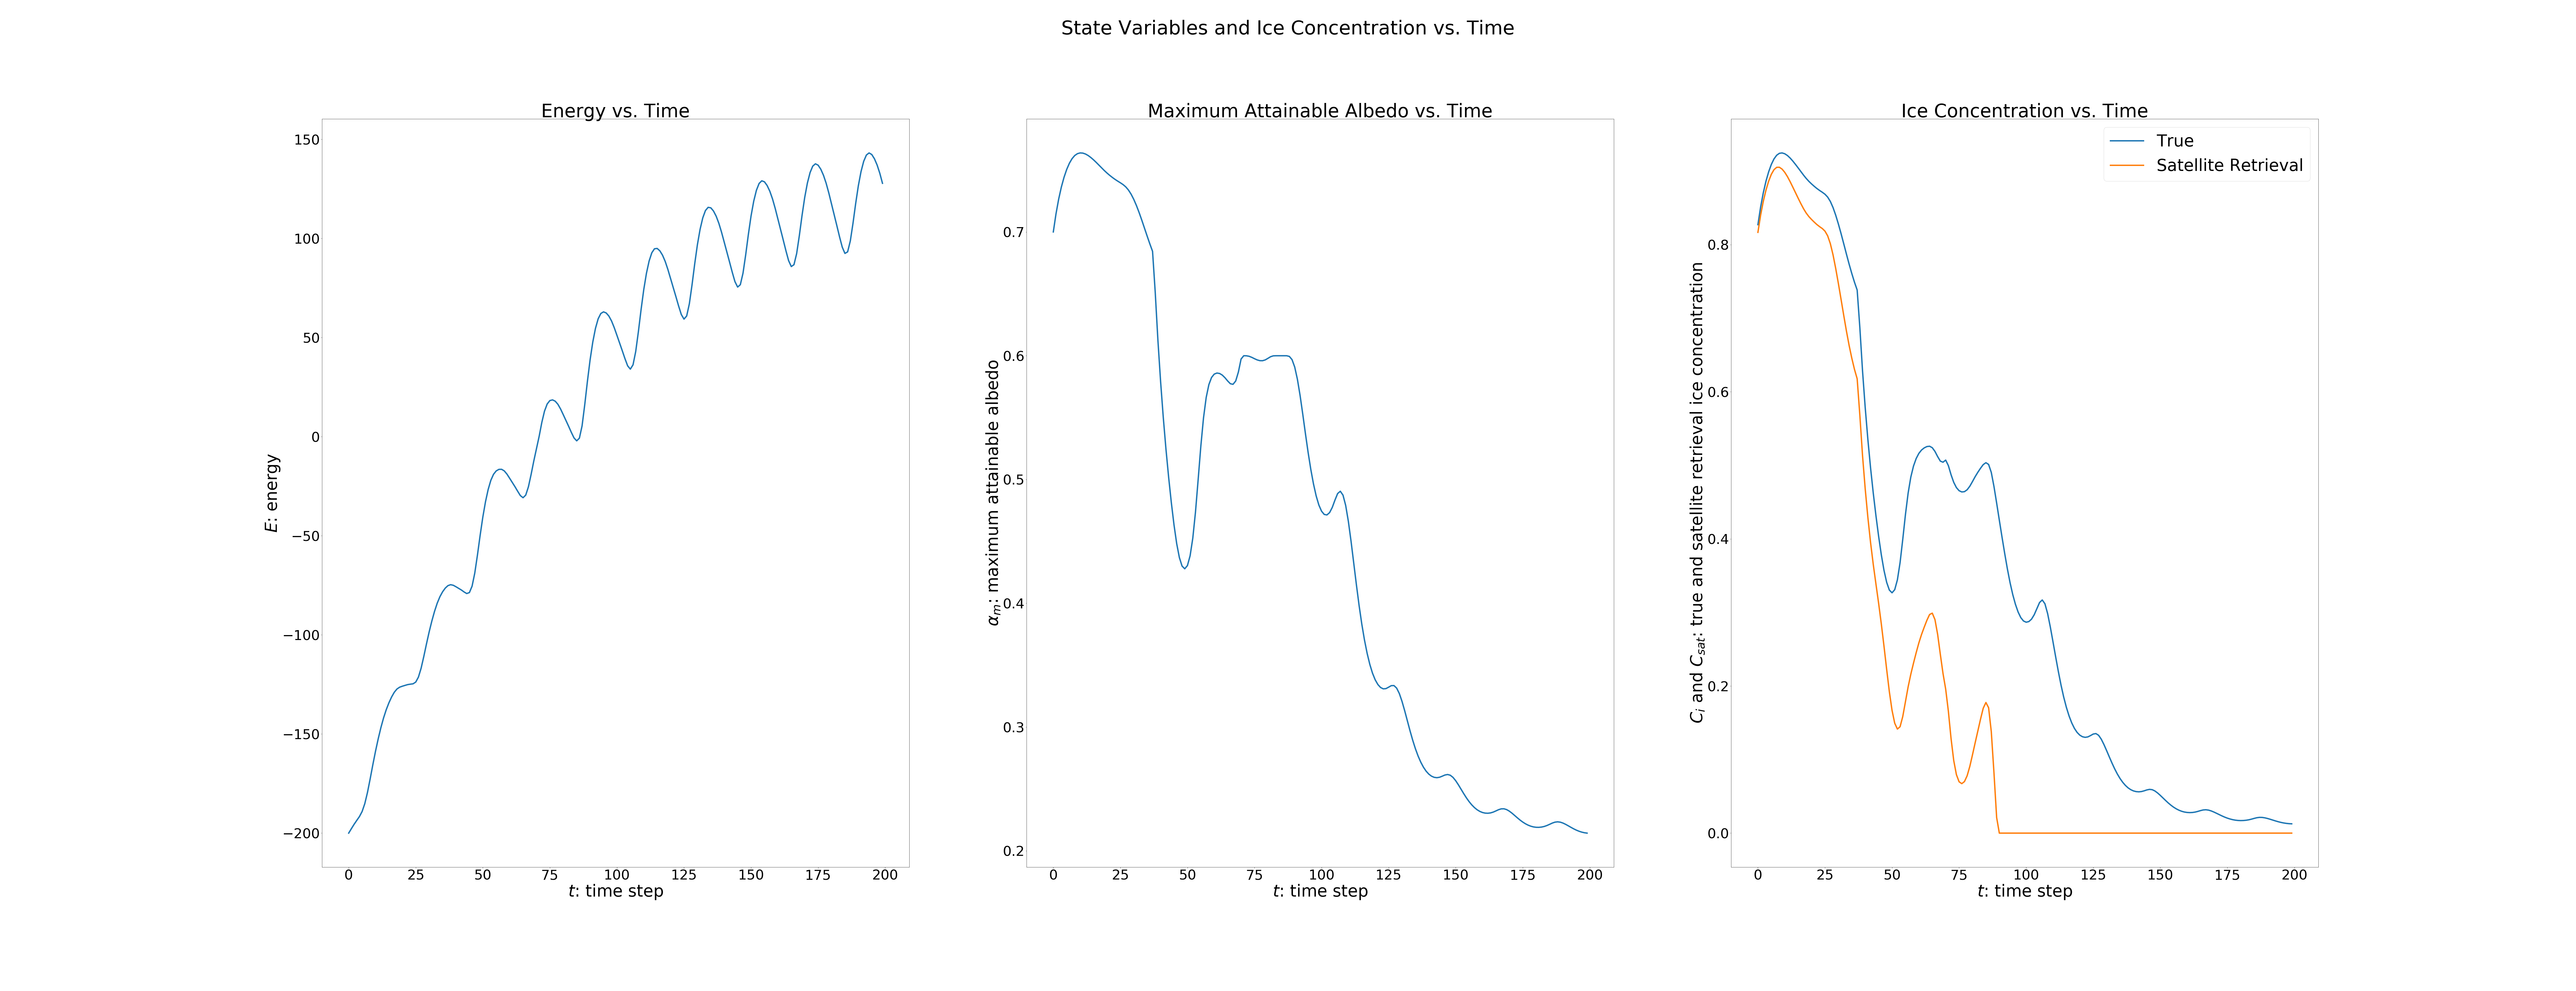
\includegraphics[width=\linewidth]{Figures/StateAndConcentration.png}
\end{center}
This motivates us to construct an observation operator taking the state variable to satellite radiances with machine learning.
\end{frame}

\begin{frame}
\frametitle{Machine Learning}
\begin{itemize}
\item
Since $\cH$ is highly nonlinear, we decide to use neural network as the machine learning algorithm.
\item A single layer of neural network: $\vx_{out}=\tanh(\vW \vx_{in}+\vb)$
\item
We compose 4 layers to get the following architecture\footnote{Biases and techniques such as batch-norm and drop-out are not shown}:
\end{itemize}
\centering
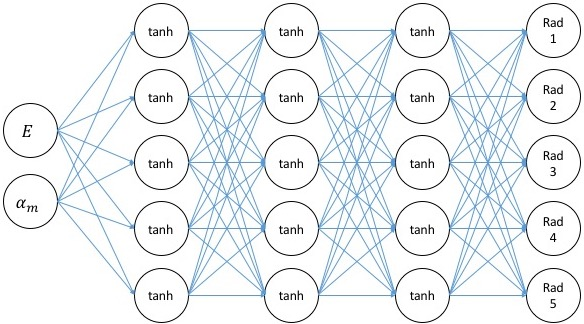
\includegraphics[width=0.6\linewidth]{Figures/FNN.jpeg}

\end{frame}

\begin{frame}
\frametitle{Data Generation}
\begin{itemize}
\item $\alpha_m$ is only meaningful in $[0.2,0.8]$. Energy lower than $-200$ would be unrealistic and uninteresting.
\begin{itemize}
	\item $\cH_{\text{grid}}$: A benchmark model trained on $120\times 180$ uniform grid data points in the state space $[0.2,0.8]\times [-200,250]$.
	\item $\cH_{\text{ML}}$: The model that mimics what we would get with the real world data, trained on trajectories in the phase space.
\end{itemize}
\item Real data comes with error, so we need to add error to the generated observations. For each of the 5 radiances, we add Gaussian error with standard deviation proportional to the mean absolute value of that radiance, i.e. $\tilde{y}_{ij} = y_{ij} + \cN(0,\lambda \bar{y}_j)$, where $\bar{y}_j =\frac{1}{n} \sum_{i=1}^n | y_{ij} |$.\par
\item We use different values of $\lambda$ from $0\%$ to $60\%$ to investigate the robustness of machine learning algorithm to error in training data.
\end{itemize}
\end{frame}

\begin{frame}
\frametitle{Evaluation}
The following figure compares the machine learning predictions with the truth and noisy data with $\lambda=40\%$.
\begin{center}
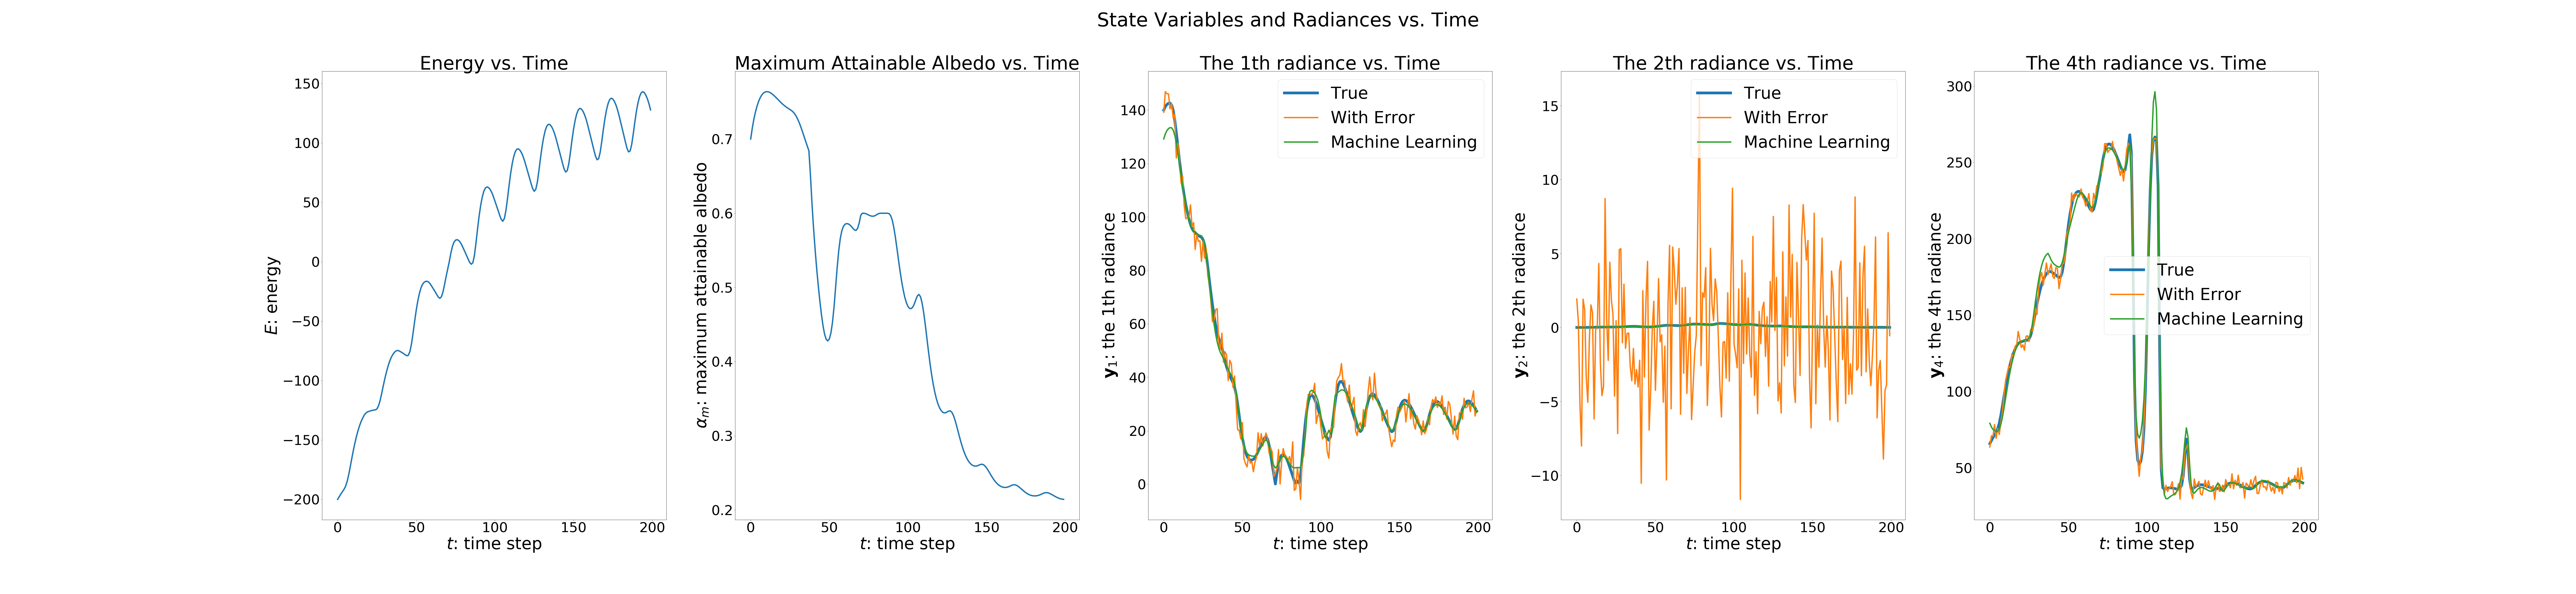
\includegraphics[width=\linewidth]{Figures/StateAndRadiances.png}
\end{center}
\begin{itemize}
\item It seems that machine learning is able to average out the noise and discover the real patter. For most values, machine learning prediction is very close to the true value.
\item In fact, through experiment, we found out that, with appropriate techniques and sufficient data, machine learning is not severely affected by the amount of noise in the training data. The model trained with $\lambda=60\%$ is only slightly worse than the model trained with $\lambda=0\%$.
\end{itemize}
\end{frame}

\begin{frame}
\frametitle{Effect of Data Density}
\begin{itemize}
	\item For the equilibrium states, where sufficient training data exists, our model tends to perform quite well.
	\item For the transient state, where training data is extremely sparse, the prediction does not make much sense.
\end{itemize}
\begin{columns}
\begin{column}{0.5\linewidth}
\centering
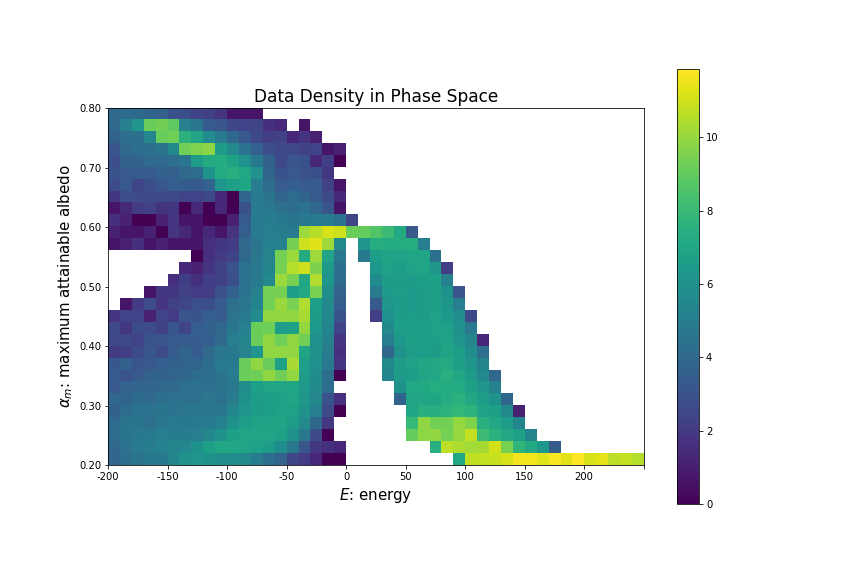
\includegraphics[width=\linewidth]{Figures/DensityMatrix.png}
\end{column}
\begin{column}{0.5\linewidth}
\centering
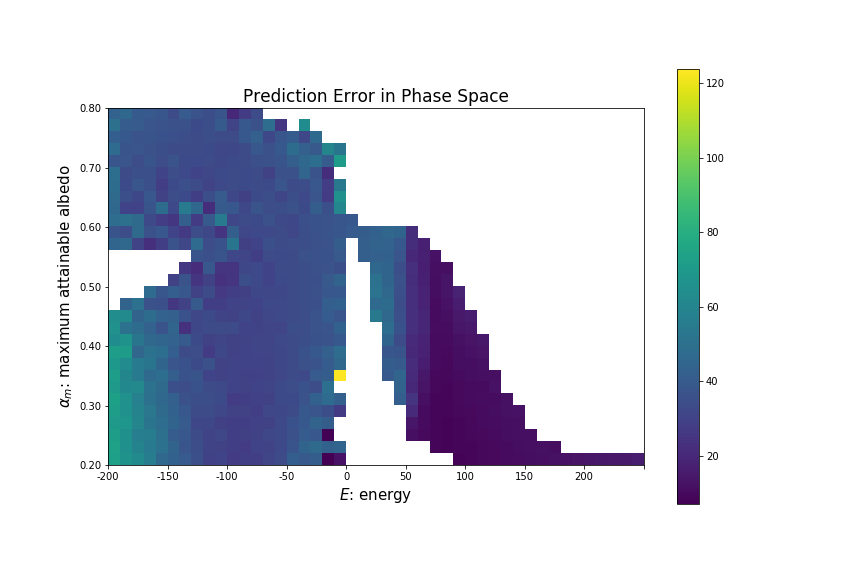
\includegraphics[width=\linewidth]{Figures/ErrorMatrix.png}
\end{column}
\end{columns}
We address this issue in data assimilation with appropriate inflation.
\end{frame}

\begin{frame}
\frametitle{Training with Sparse Data}
What if we don't have sufficient data in certain regions of interest?\par
\begin{center}
\includegraphics[width=0.8\linewidth]{Figures/sparse.png}
\end{center}
We randomly drop $95\%$ / $70\%$ of the data in the shaded region to investigate the robustness of machine learning to sparse data, and the performance of EnKF in this kind of situation.
\end{frame}

\begin{frame}
\frametitle{Training with Sparse Data: Evaluation}
With only $5\%$ of the data, our neural network starts to make mistakes.
\centering
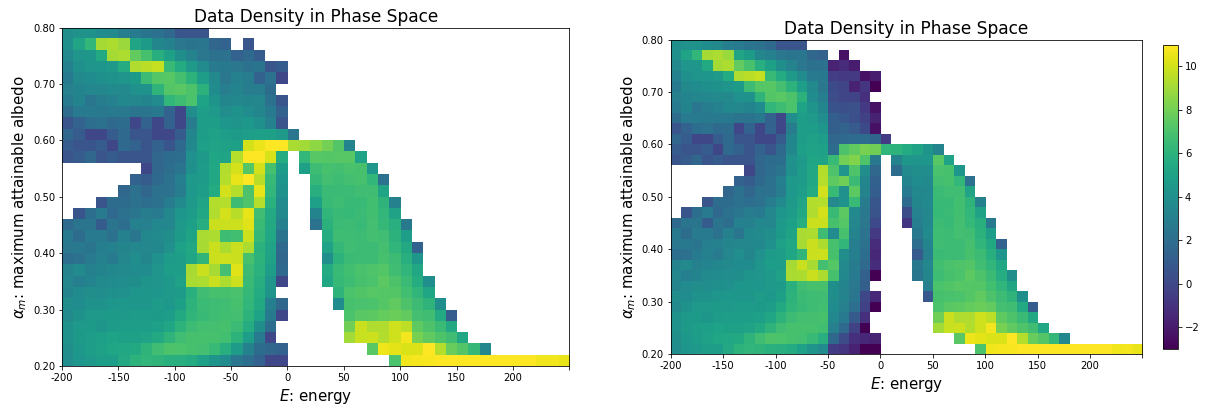
\includegraphics[width=0.8\linewidth]{Figures/DensityMatrix_sparse_comparison.png}
\centering
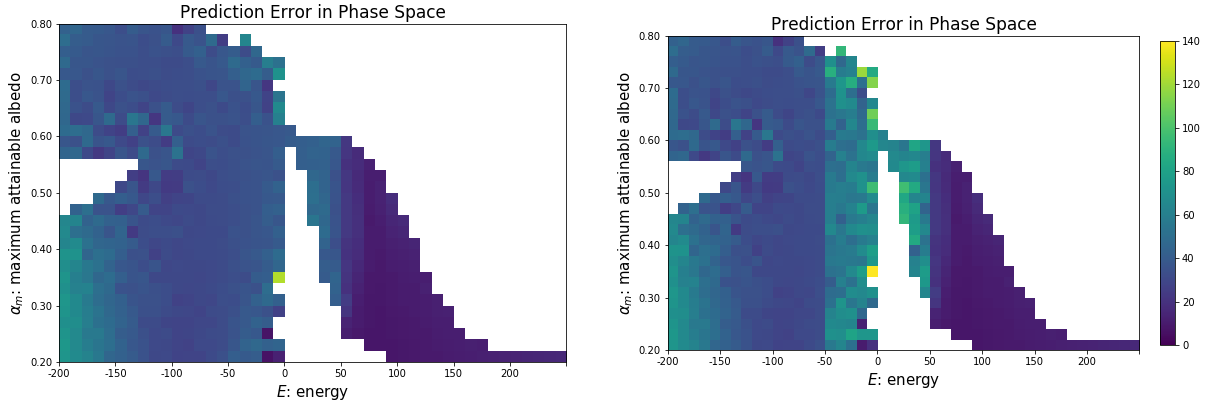
\includegraphics[width=0.8\linewidth]{Figures/ErrorMatrix_sparse_comparison.png}
\end{frame}

\begin{frame}
\frametitle{Experiment}
Experiment setup:
\begin{itemize}
	\item Initial condition: $\mx_0=[0.7,-200]$, $F_{CO_2}=60$
	\item Initial ensemble mean: $\mx_0+\cN(0,\begin{bmatrix}
	0.12 & 0 \\
	0 & 40
	\end{bmatrix})$
	\item Initial ensemble spread: $\begin{bmatrix}
	0.12 & 0 \\
	0 & 40
	\end{bmatrix}$
	\item Size of ensemble: 100
	\item Time step: $0.05 \times 200$
	\item Observation error: $20\%$ of the mean absolute value
\end{itemize}
\end{frame}

\begin{frame}
\frametitle{Results: Baseline Model}
{\setlength{\baselineskip}{0.001em}
\tiny{Machine learning model:}
\begin{center}
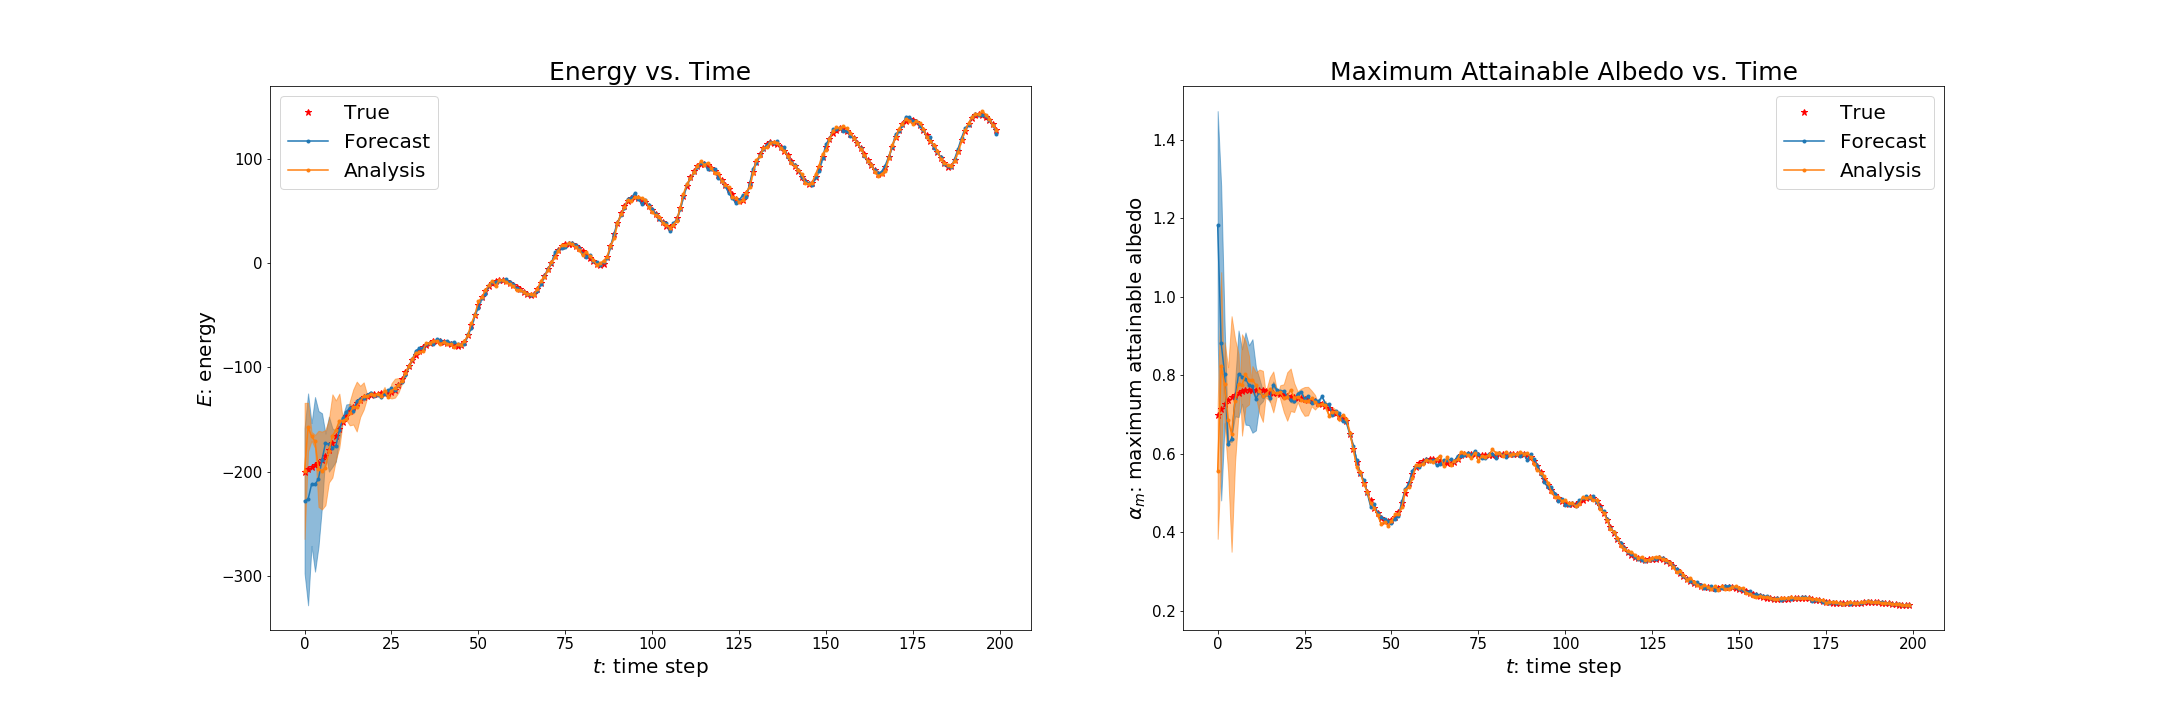
\includegraphics[width=0.85\linewidth]{Figures/H_ml_hat_grid_new.png} 
\end{center}
\tiny{True radiance operator:}
\begin{center}
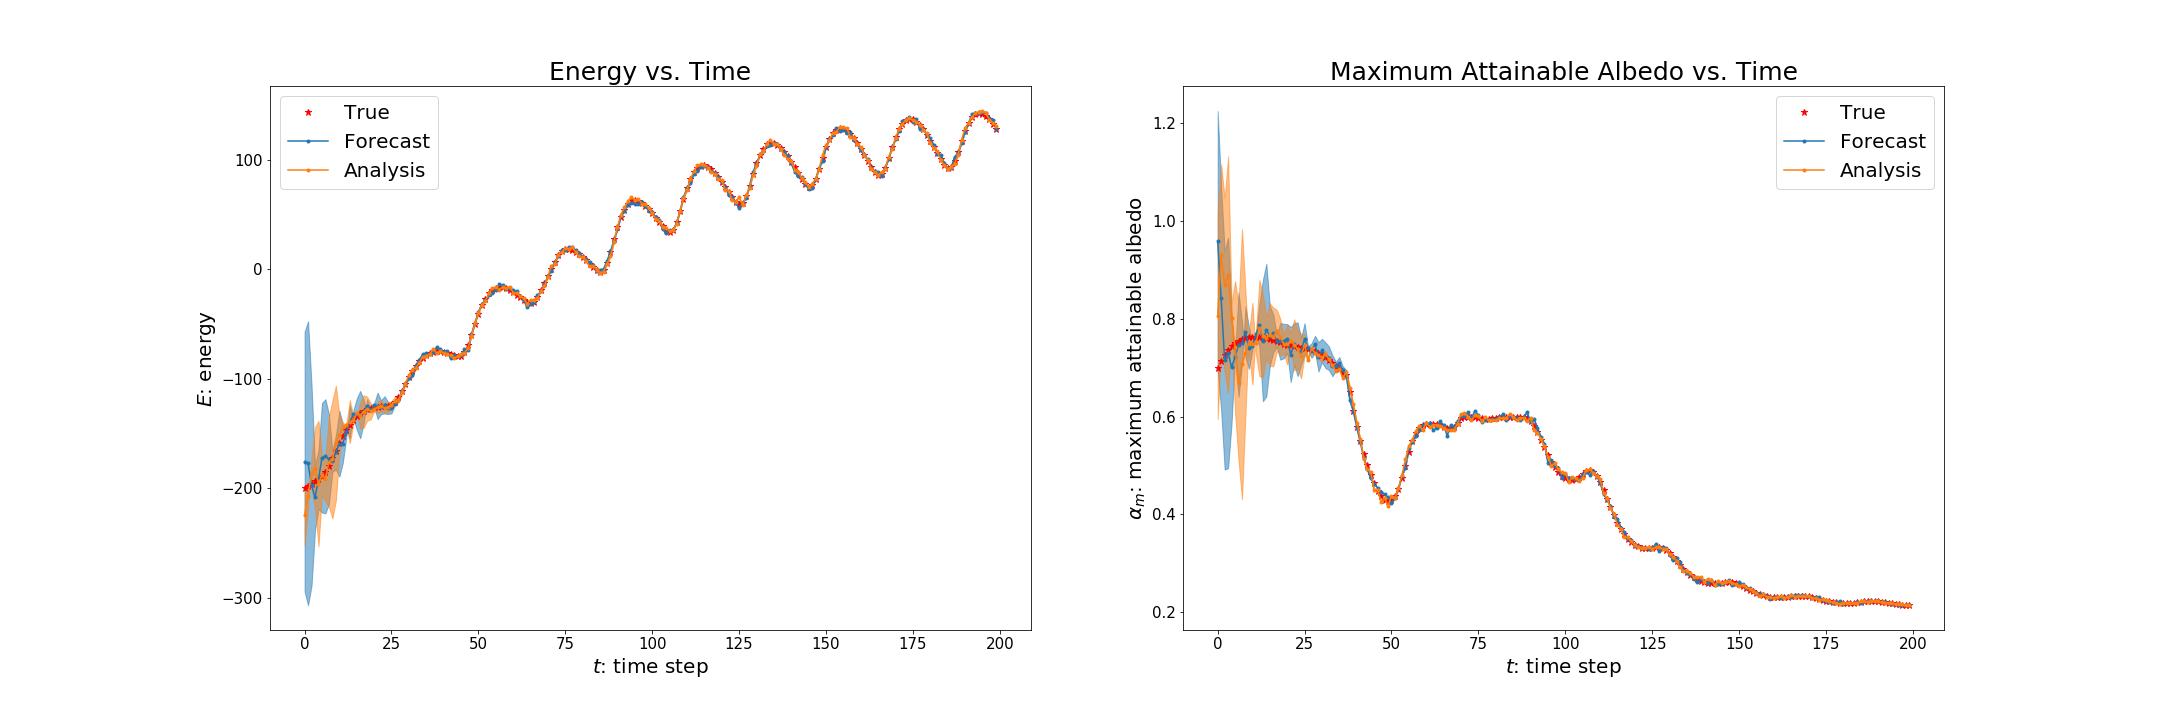
\includegraphics[width=0.85\linewidth]{Figures/H_true_new.png} 
\end{center}
}
\end{frame}

\begin{frame}
\frametitle{Results: Baseline Model}
{\setlength{\baselineskip}{0.001em}
\tiny{Machine learning model:}
\begin{center}
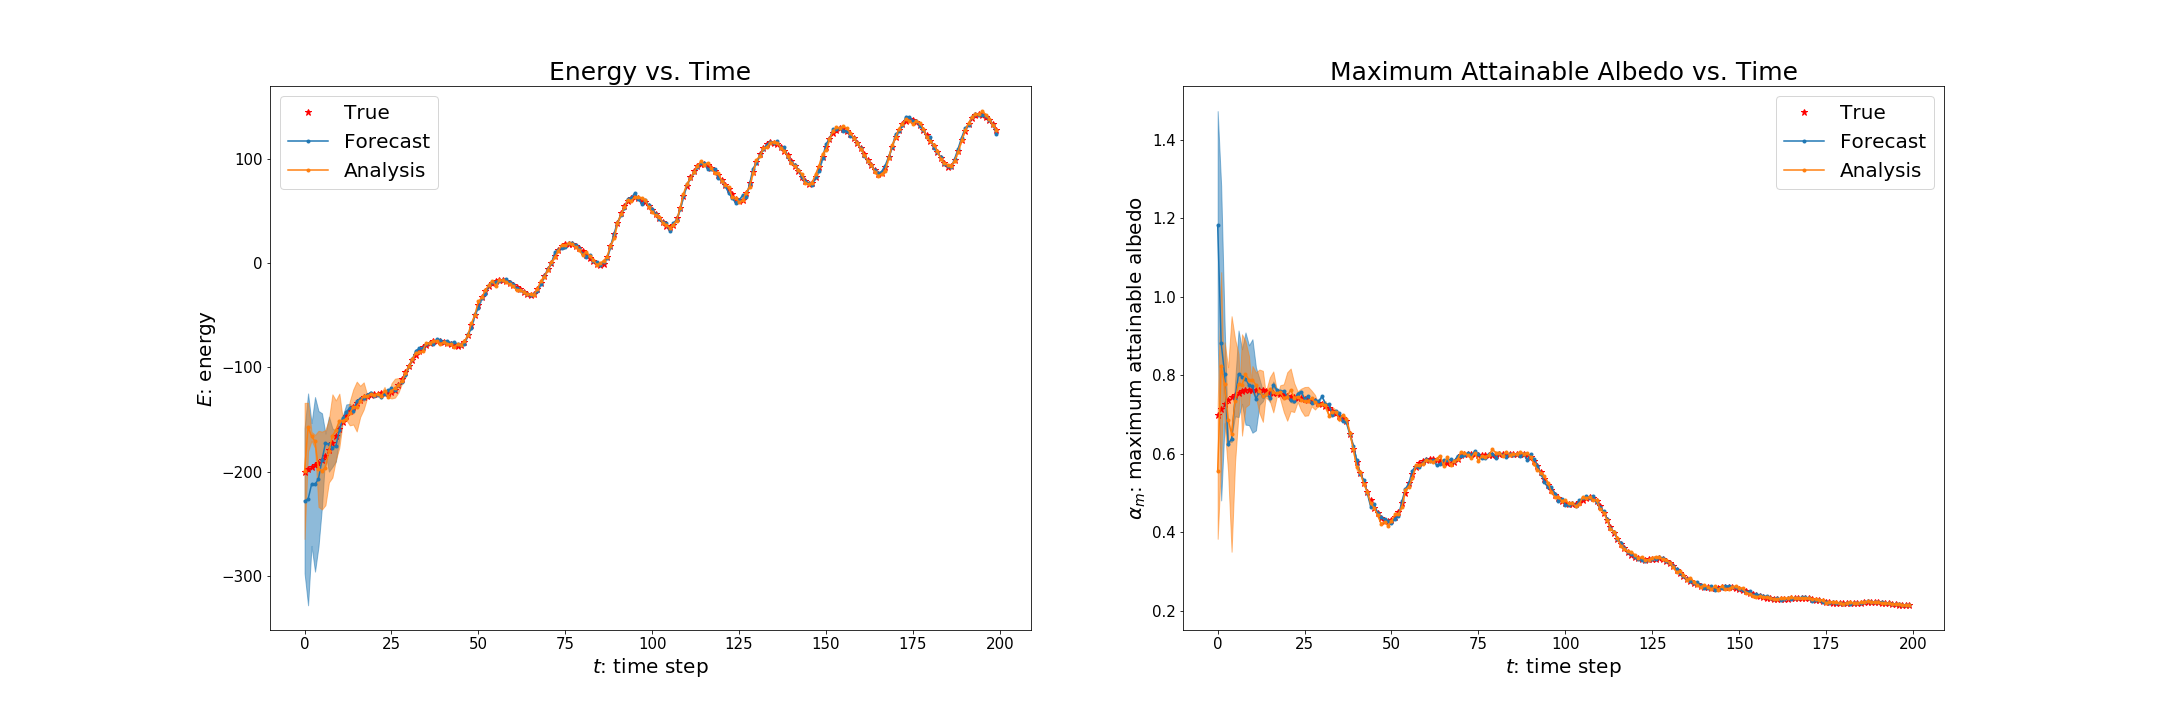
\includegraphics[width=0.85\linewidth]{Figures/H_ml_hat_grid_new.png} 
\end{center}
\tiny{Retrieval algorithm:}
\begin{center}
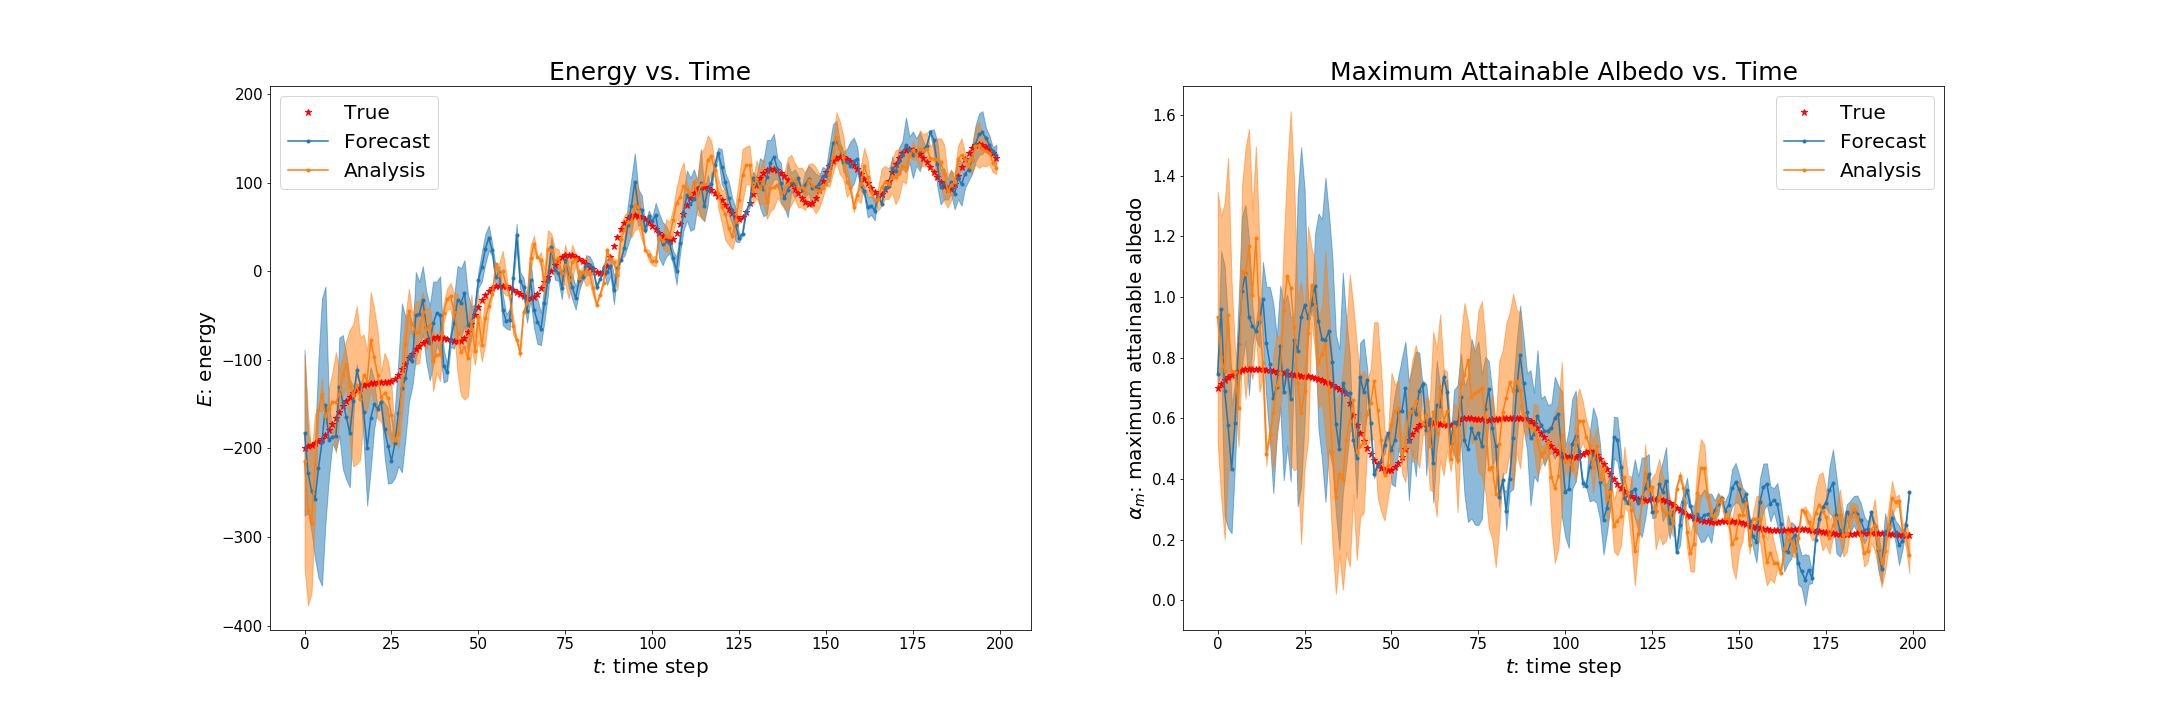
\includegraphics[width=0.85\linewidth]{Figures/H_retrieval_new.png} 
\end{center}
}
\end{frame}

\begin{frame}
\frametitle{Results: Realistic Model}
{\setlength{\baselineskip}{0.001em}
\tiny{Machine learning model with trajectory training data:}
\begin{center}
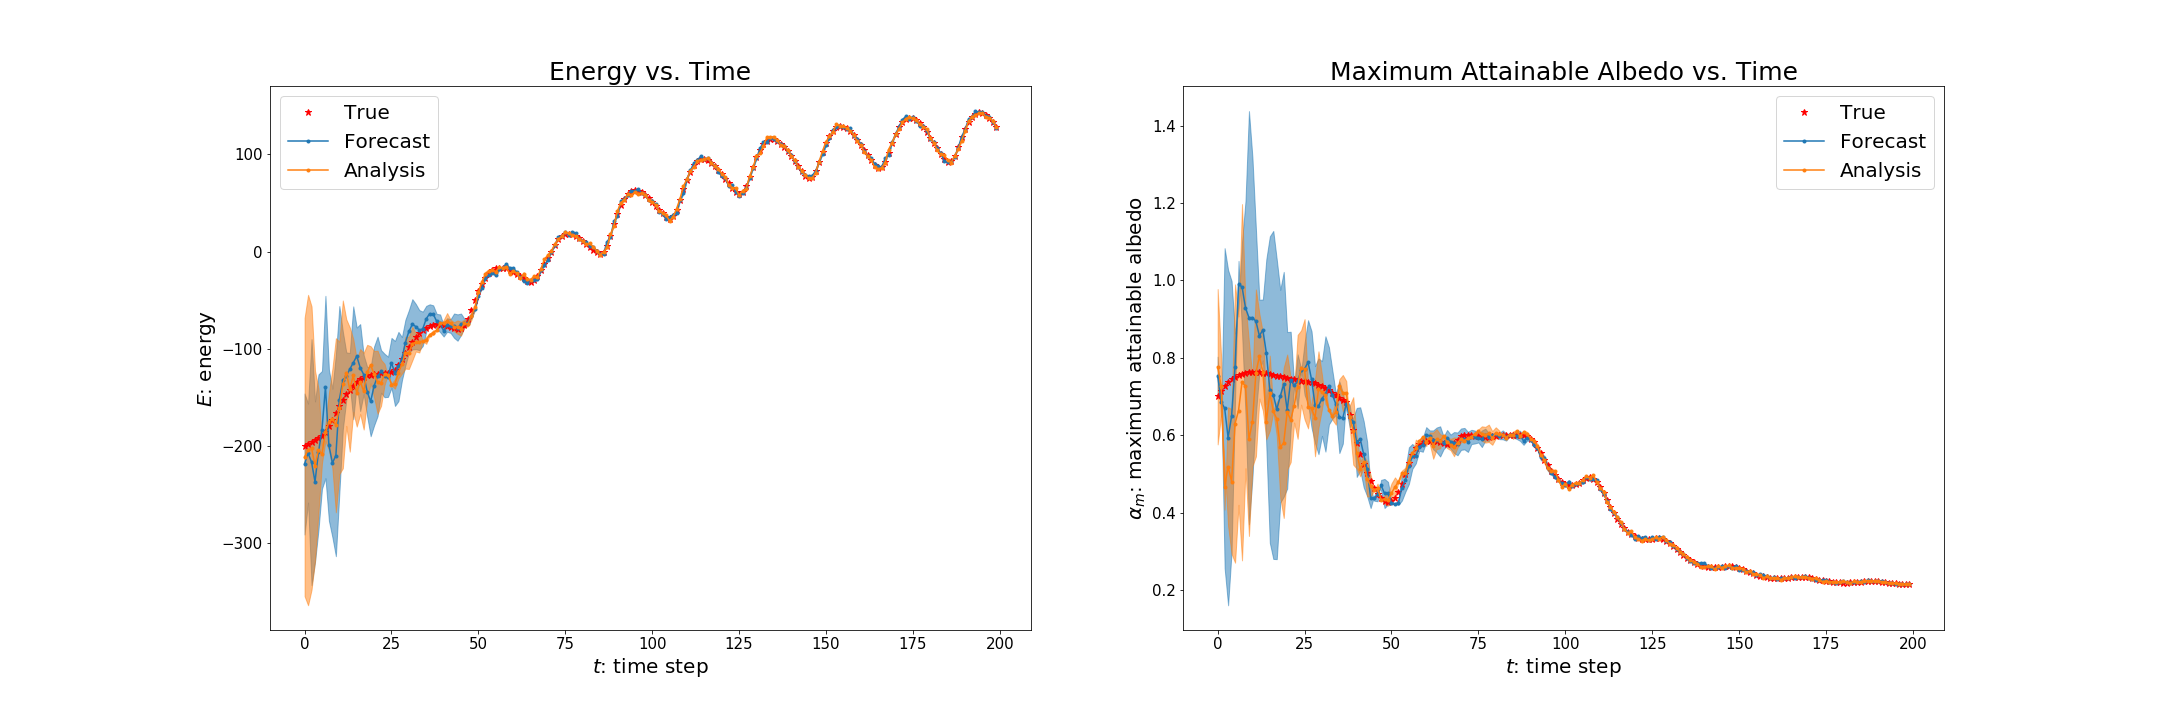
\includegraphics[width=0.85\linewidth]{Figures/H_ml_hat_new.png} 
\end{center}
\tiny{Machine learning model with grid training data:}
\begin{center}
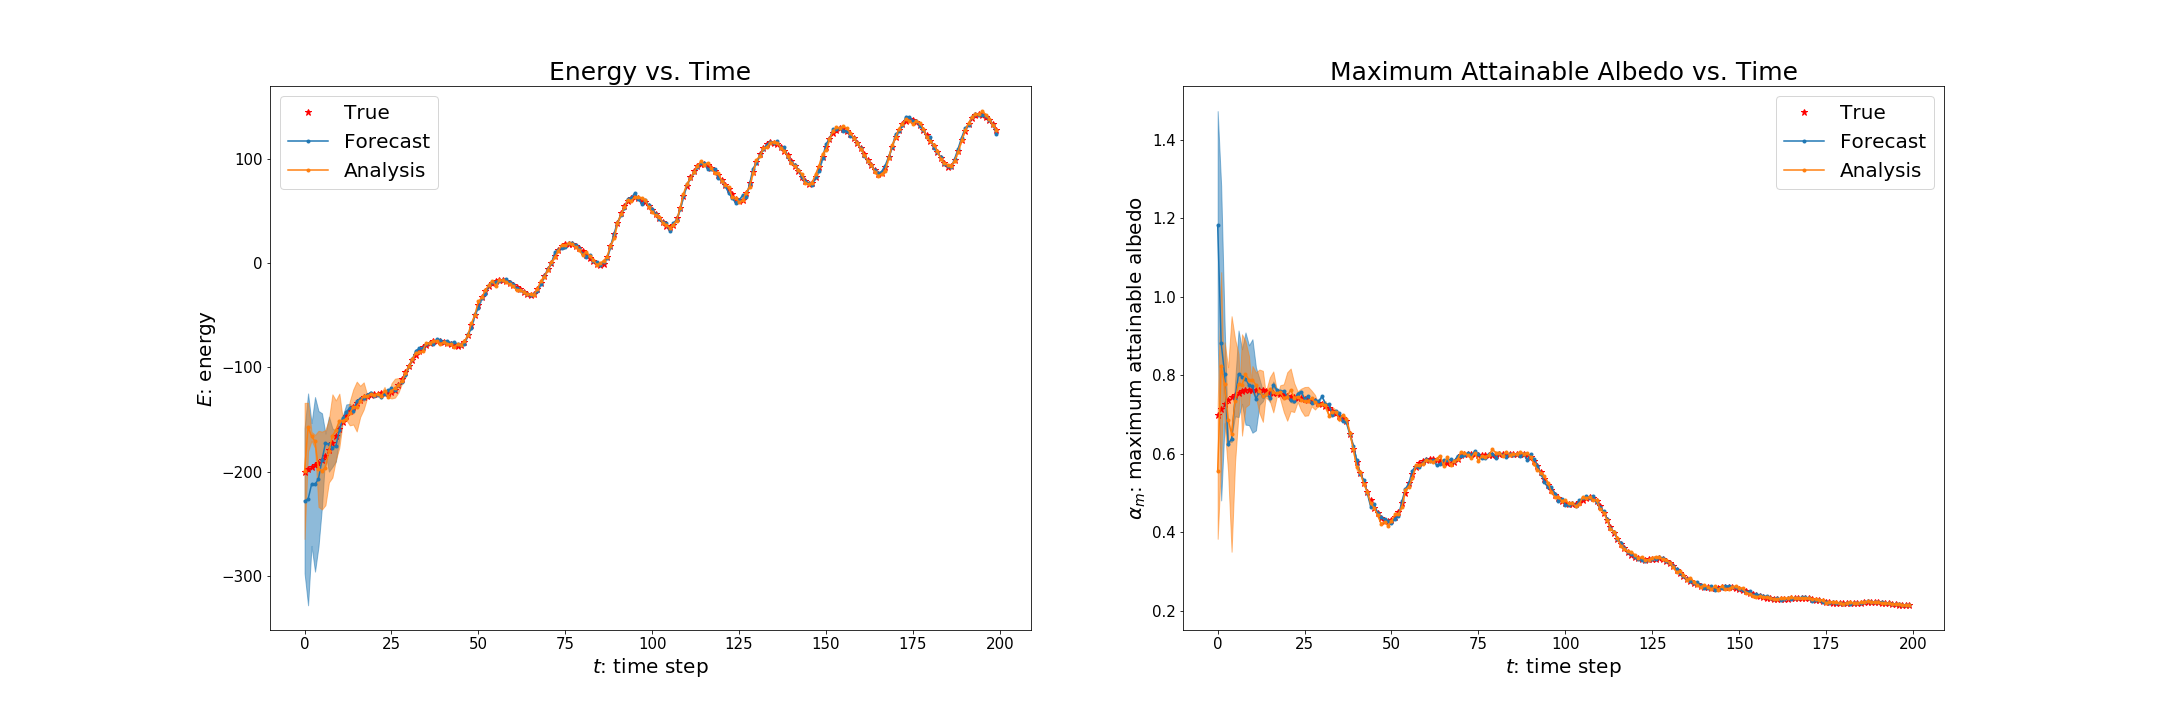
\includegraphics[width=0.85\linewidth]{Figures/H_ml_hat_grid_new.png} 
\end{center}
}
\end{frame}

\begin{frame}
\frametitle{Results: Realistic Model}
\centering
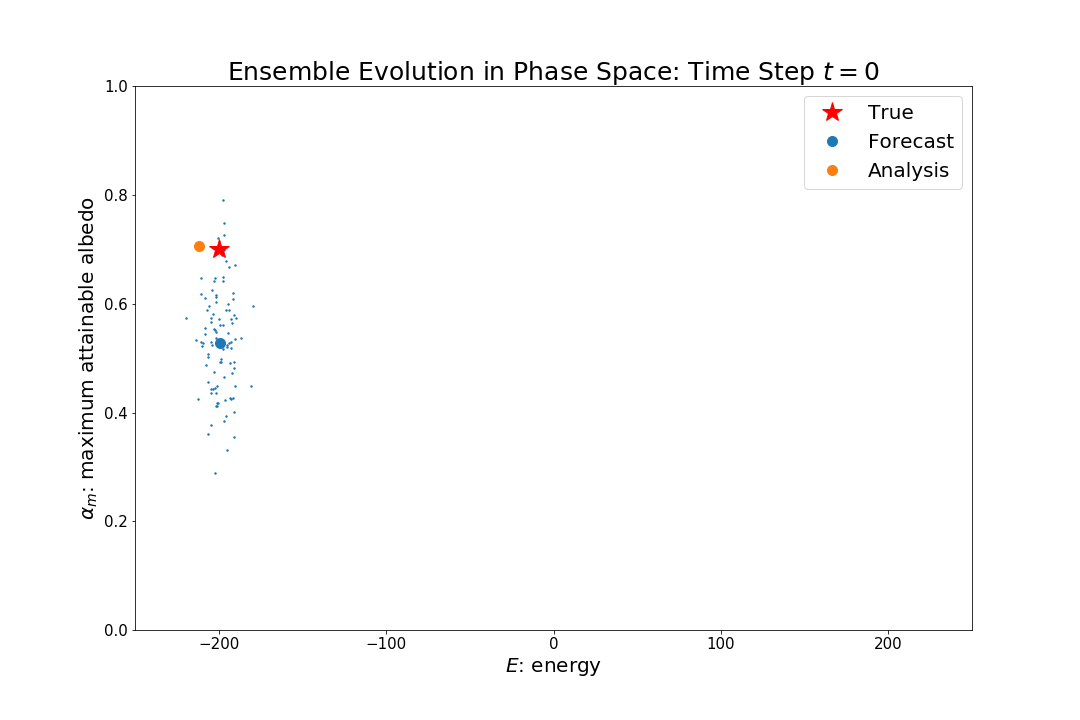
\includegraphics[width=\linewidth]{Figures/EnsembleEvolution_forecast_t=0.png}
\end{frame}
\begin{frame}
\frametitle{Results: Realistic Model}
\centering
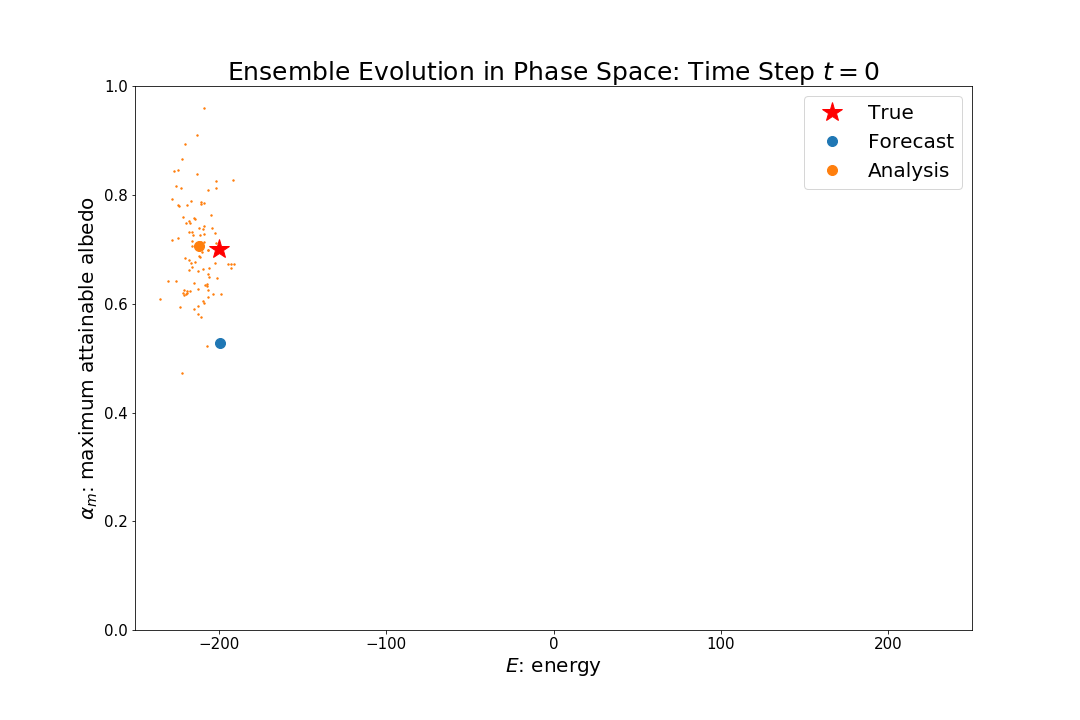
\includegraphics[width=\linewidth]{Figures/EnsembleEvolution_analysis_t=0.png}
\end{frame}
\begin{frame}
\frametitle{Results: Realistic Model}
\centering
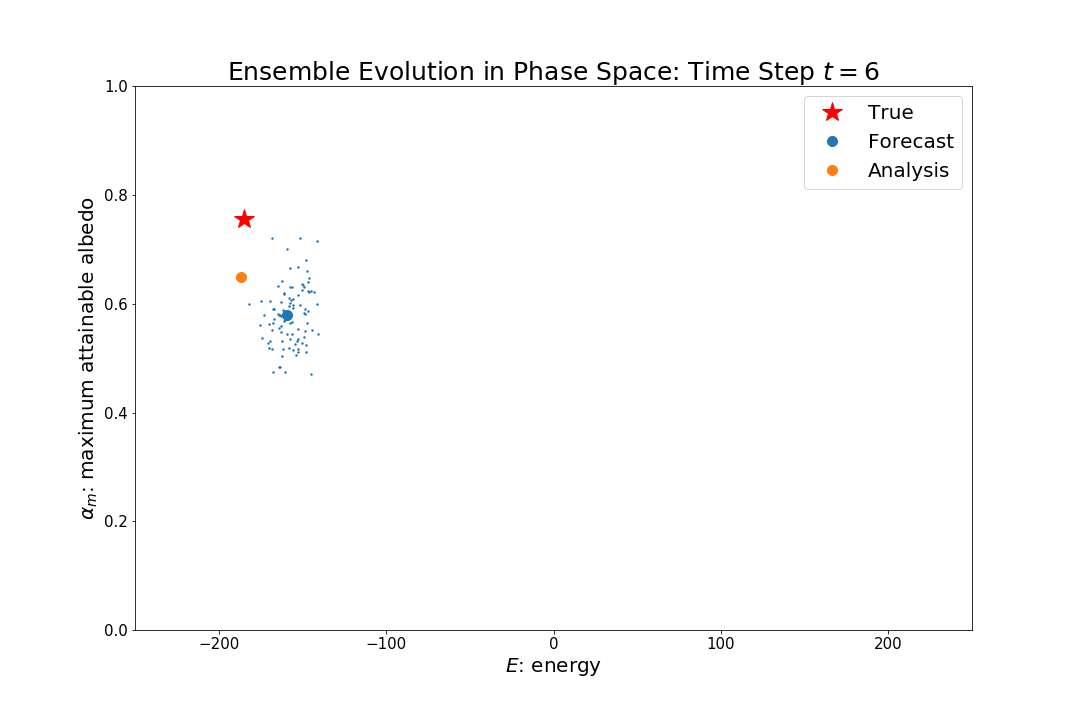
\includegraphics[width=\linewidth]{Figures/EnsembleEvolution_forecast_t=6.png}
\end{frame}
\begin{frame}
\frametitle{Results: Realistic Model}
\centering
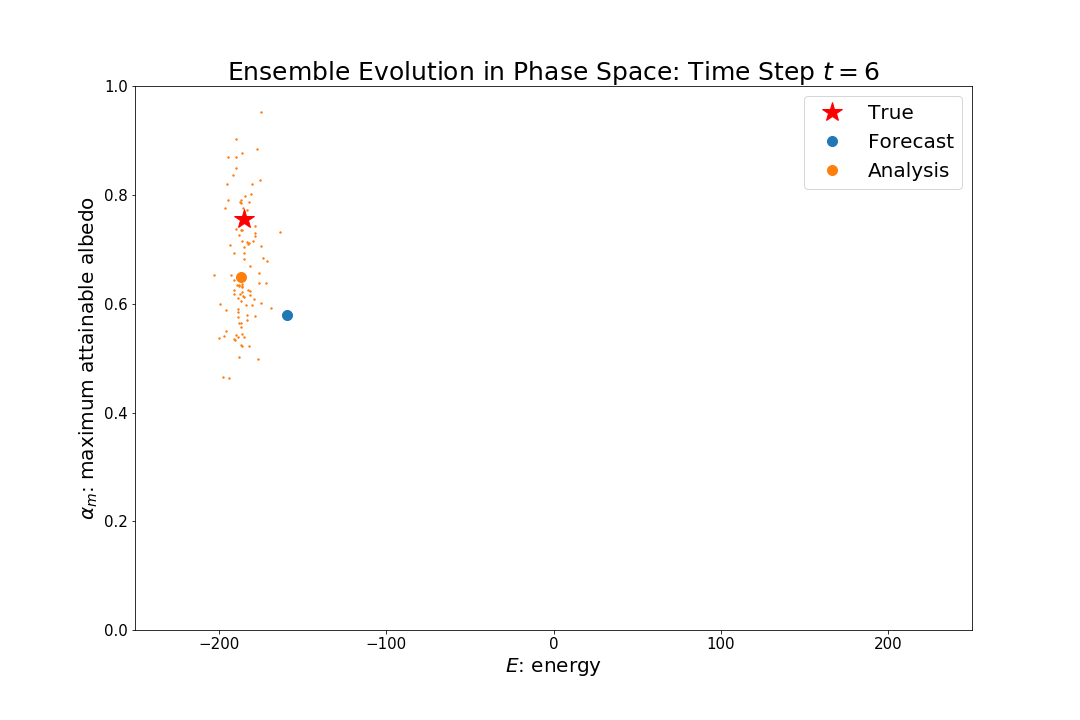
\includegraphics[width=\linewidth]{Figures/EnsembleEvolution_analysis_t=6.png}
\end{frame}
\begin{frame}
\frametitle{Results: Realistic Model}
\centering
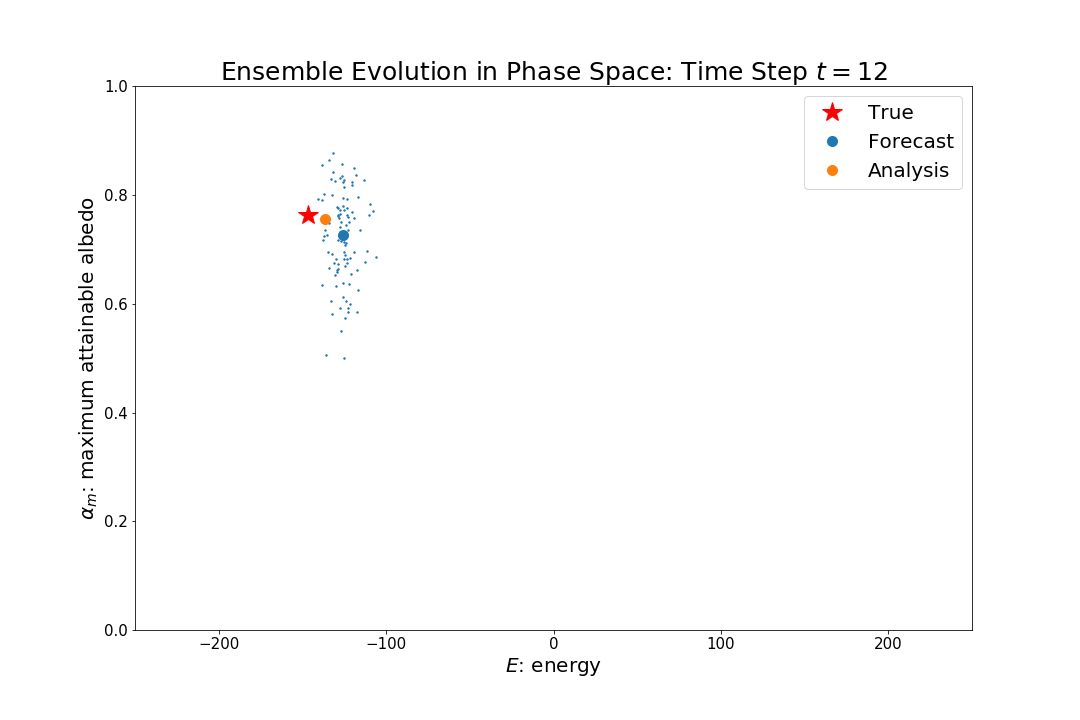
\includegraphics[width=\linewidth]{Figures/EnsembleEvolution_forecast_t=12.png}
\end{frame}
\begin{frame}
\frametitle{Results: Realistic Model}
\centering
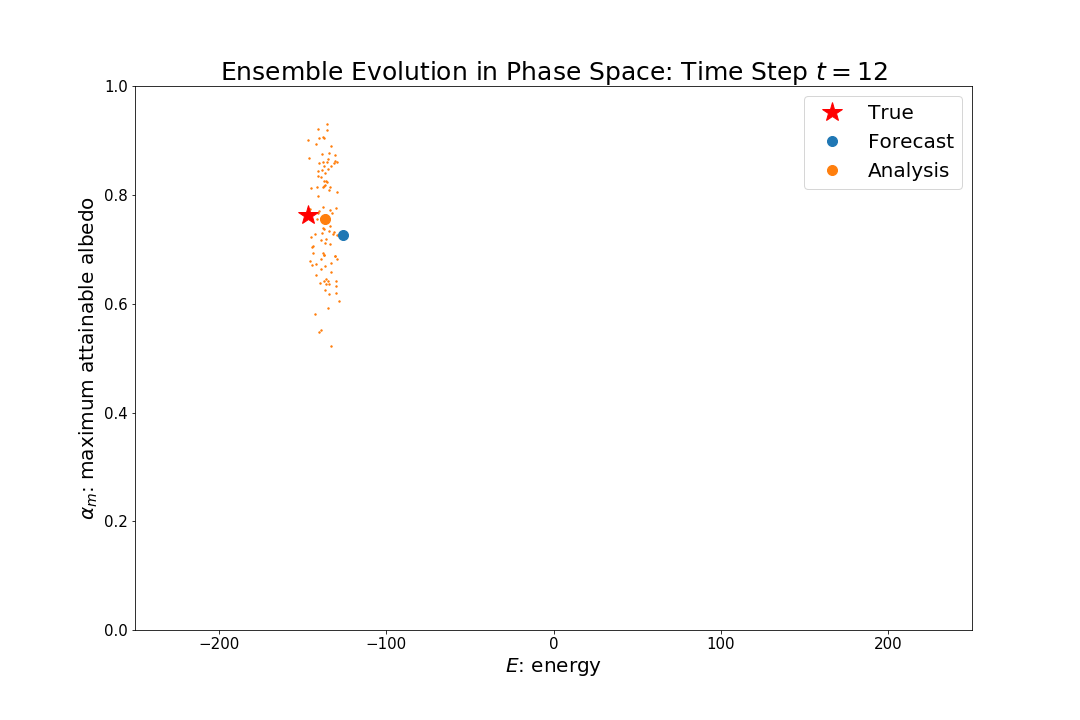
\includegraphics[width=\linewidth]{Figures/EnsembleEvolution_analysis_t=12.png}
\end{frame}
\begin{frame}
\frametitle{Results: Realistic Model}
\centering
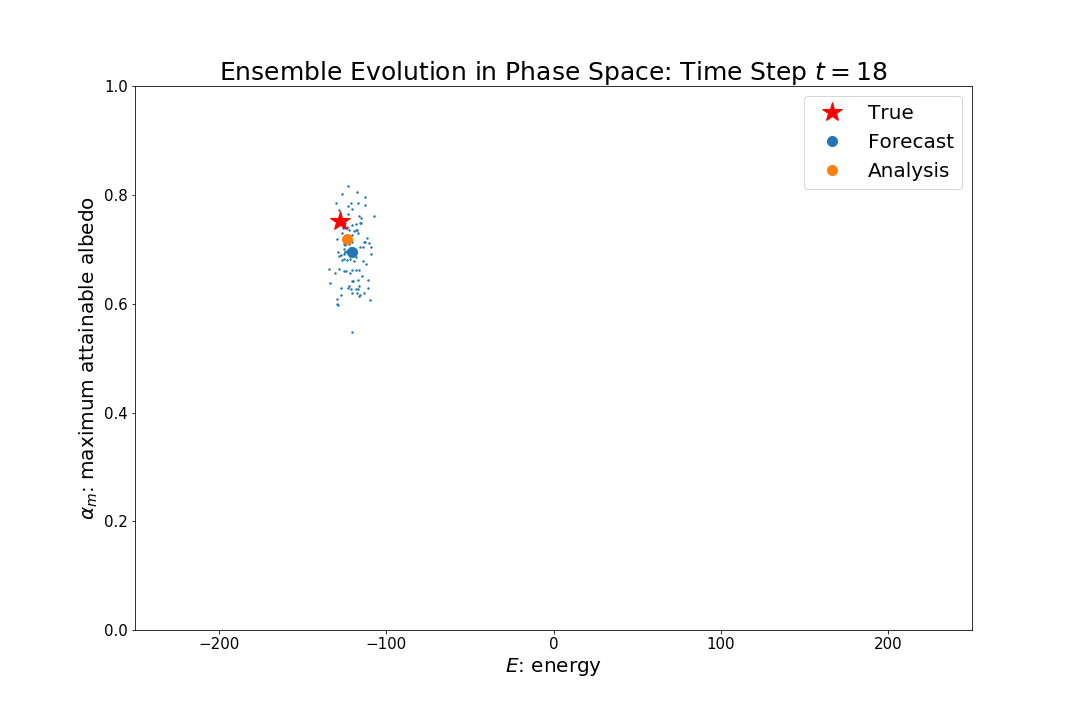
\includegraphics[width=\linewidth]{Figures/EnsembleEvolution_forecast_t=18.png}
\end{frame}
\begin{frame}
\frametitle{Results: Realistic Model}
\centering
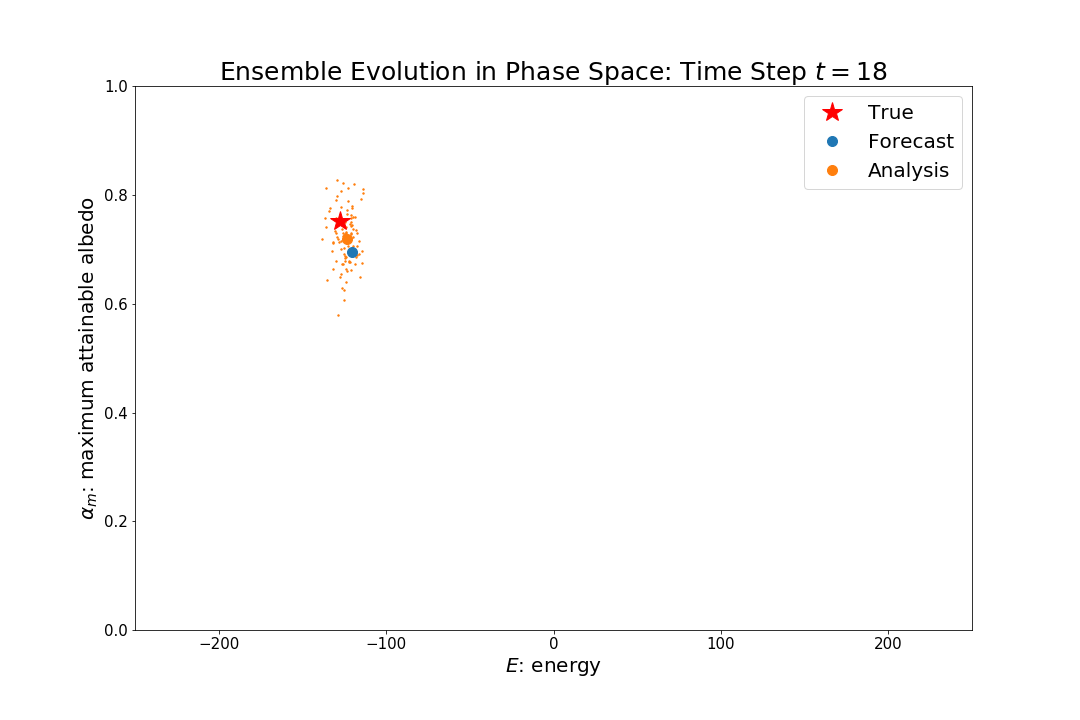
\includegraphics[width=\linewidth]{Figures/EnsembleEvolution_analysis_t=18.png}
\end{frame}
\begin{frame}
\frametitle{Results: Realistic Model}
\centering
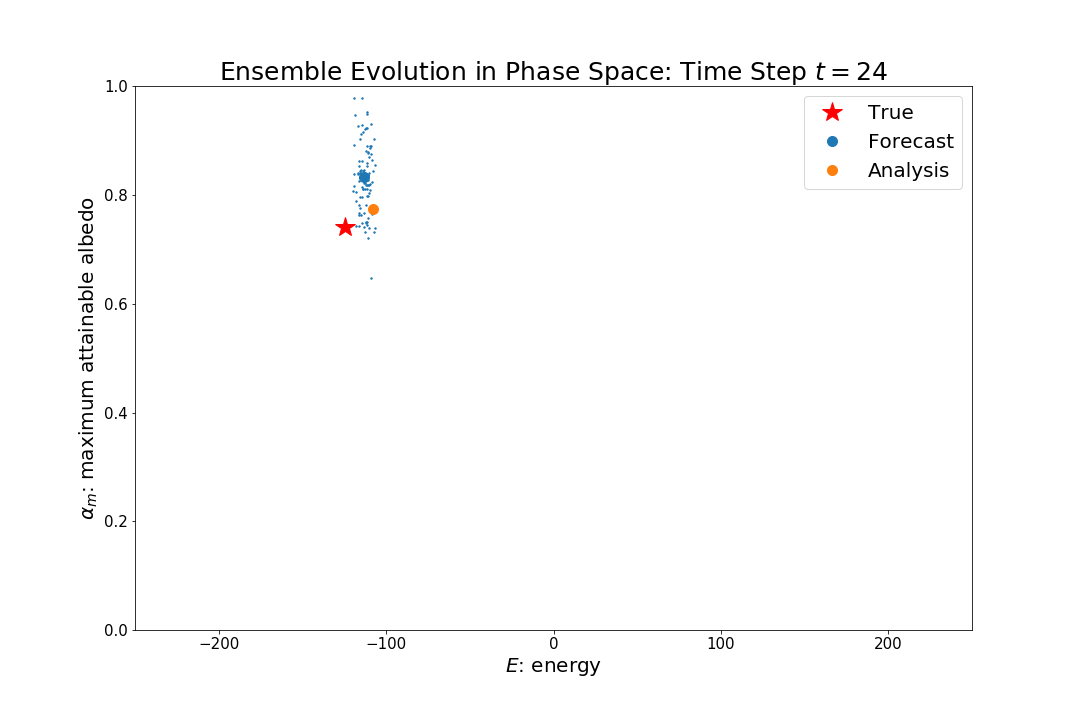
\includegraphics[width=\linewidth]{Figures/EnsembleEvolution_forecast_t=24.png}
\end{frame}
\begin{frame}
\frametitle{Results: Realistic Model}
\centering
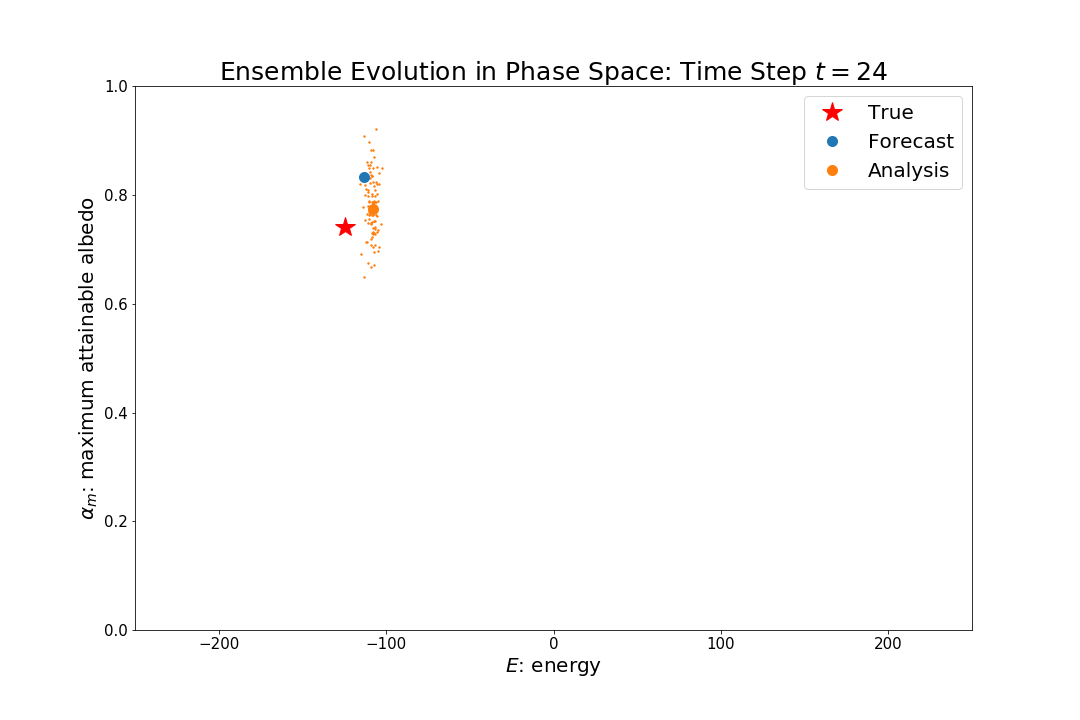
\includegraphics[width=\linewidth]{Figures/EnsembleEvolution_analysis_t=24.png}
\end{frame}
\begin{frame}
\frametitle{Results: Realistic Model}
\centering
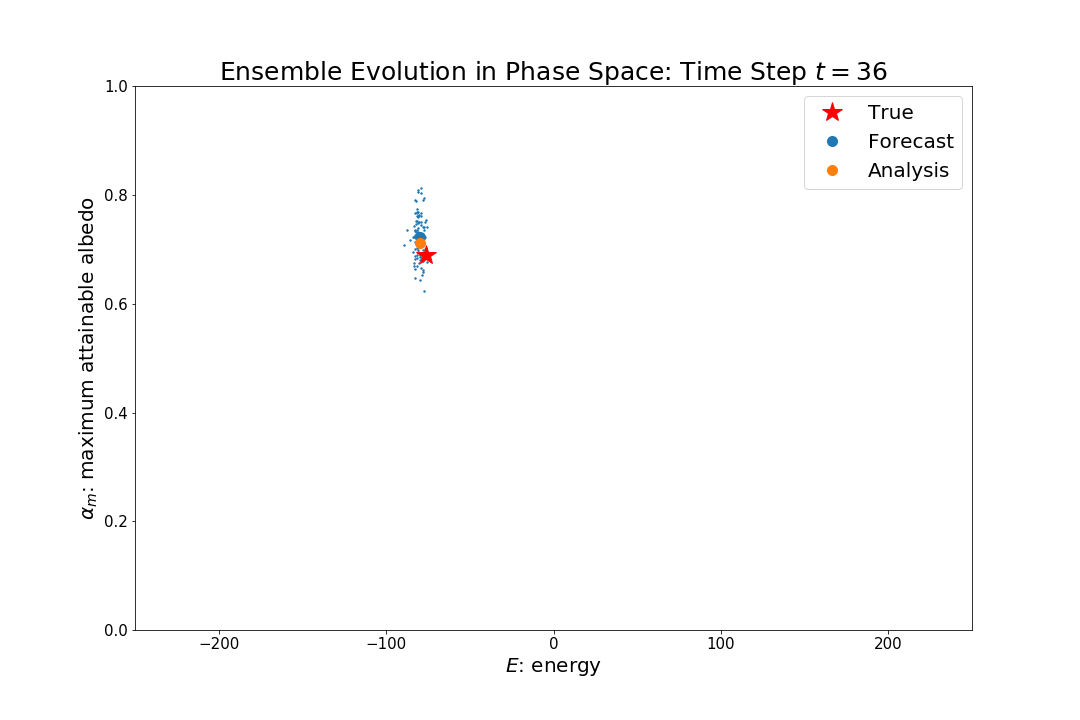
\includegraphics[width=\linewidth]{Figures/EnsembleEvolution_forecast_t=36.png}
\end{frame}
\begin{frame}
\frametitle{Results: Realistic Model}
\centering
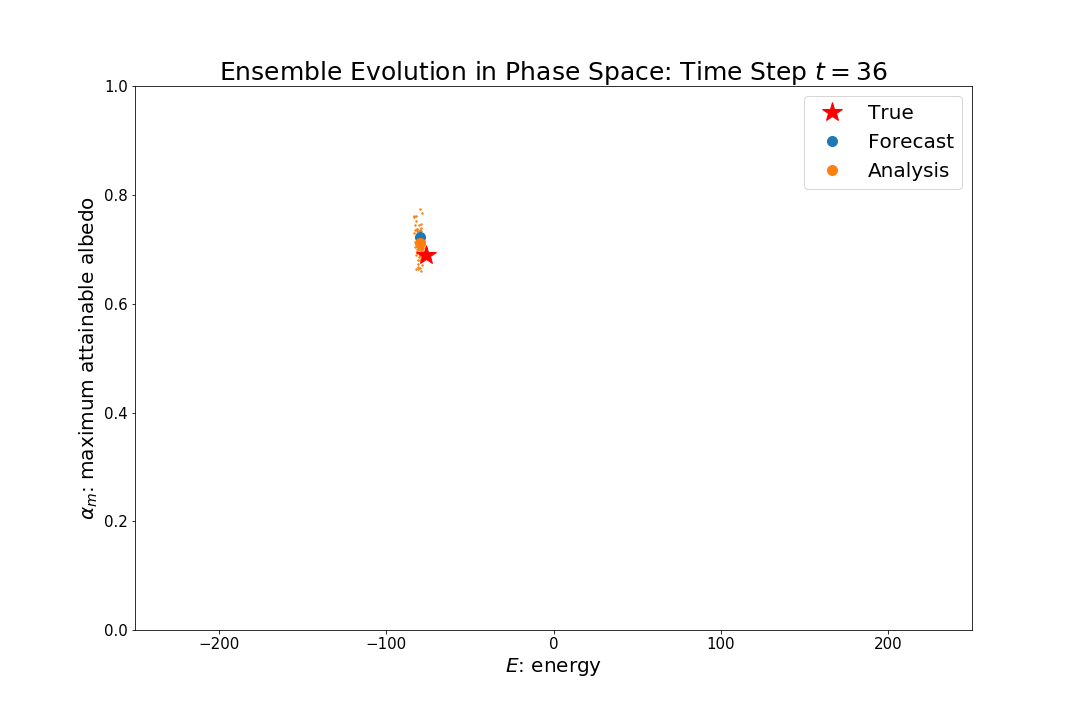
\includegraphics[width=\linewidth]{Figures/EnsembleEvolution_analysis_t=36.png}
\end{frame}
\begin{frame}
\frametitle{Results: Realistic Model}
\centering
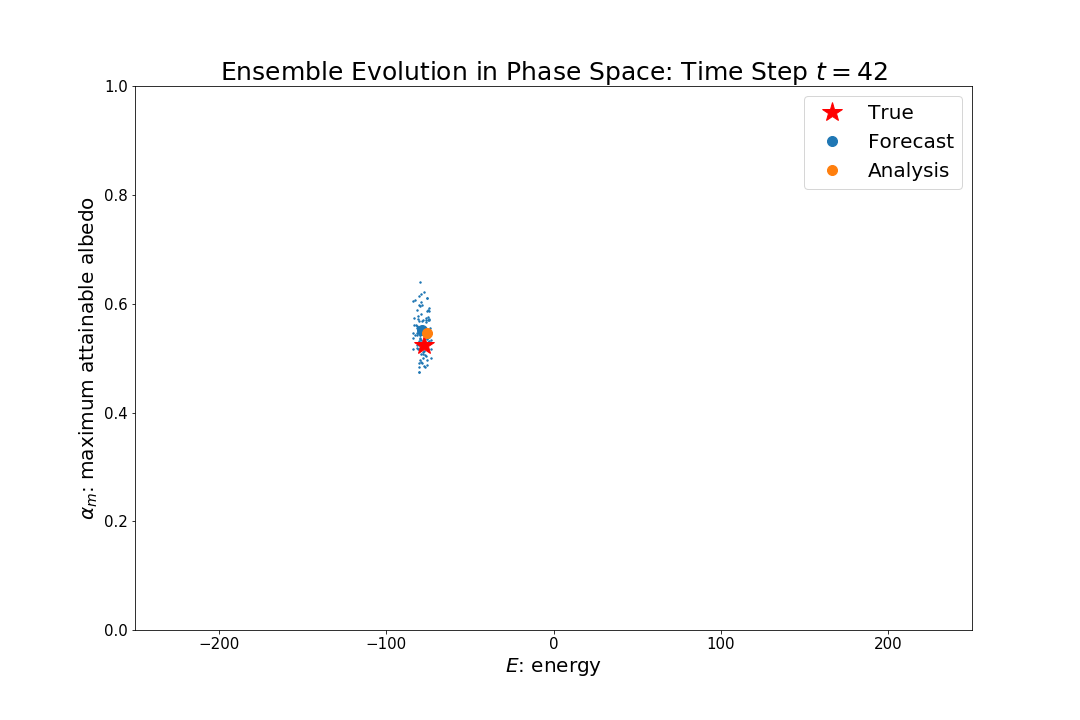
\includegraphics[width=\linewidth]{Figures/EnsembleEvolution_forecast_t=42.png}
\end{frame}
\begin{frame}
\frametitle{Results: Realistic Model}
\centering
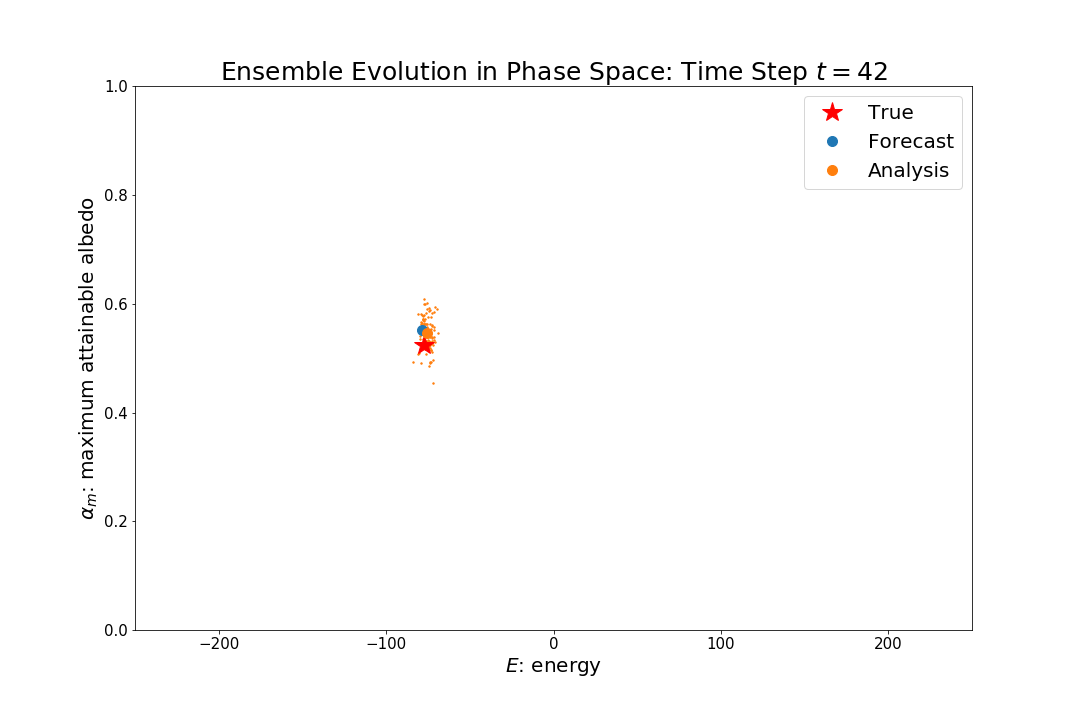
\includegraphics[width=\linewidth]{Figures/EnsembleEvolution_analysis_t=42.png}
\end{frame}
\begin{frame}
\frametitle{Results: Realistic Model}
\centering
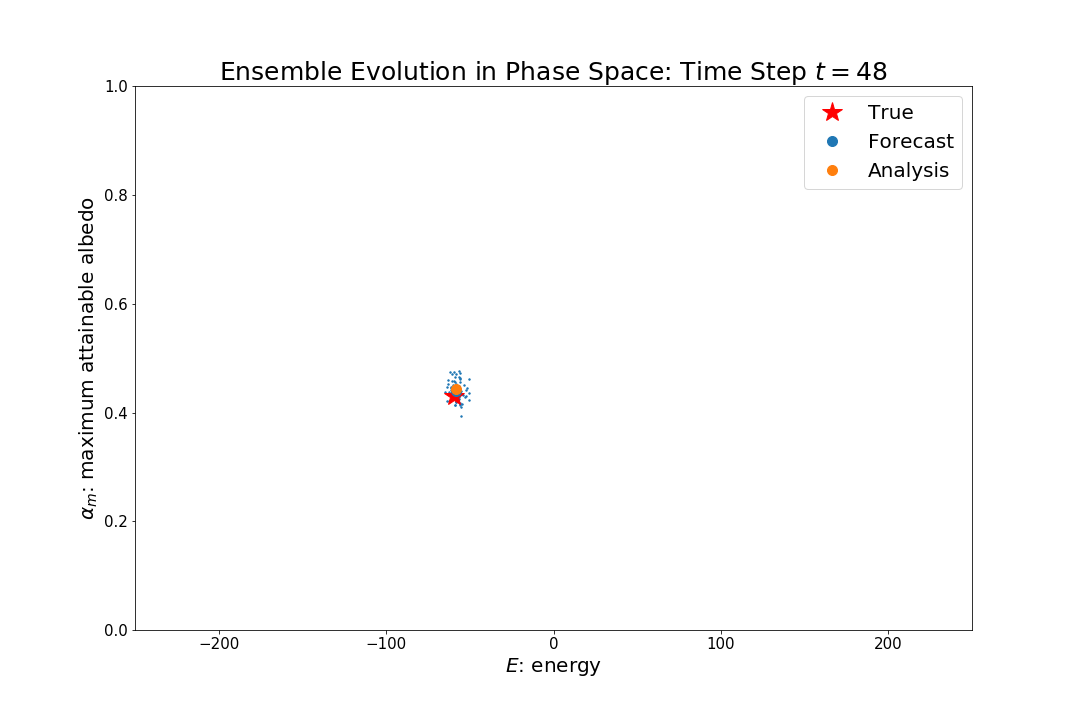
\includegraphics[width=\linewidth]{Figures/EnsembleEvolution_forecast_t=48.png}
\end{frame}
\begin{frame}
\frametitle{Results: Realistic Model}
\centering
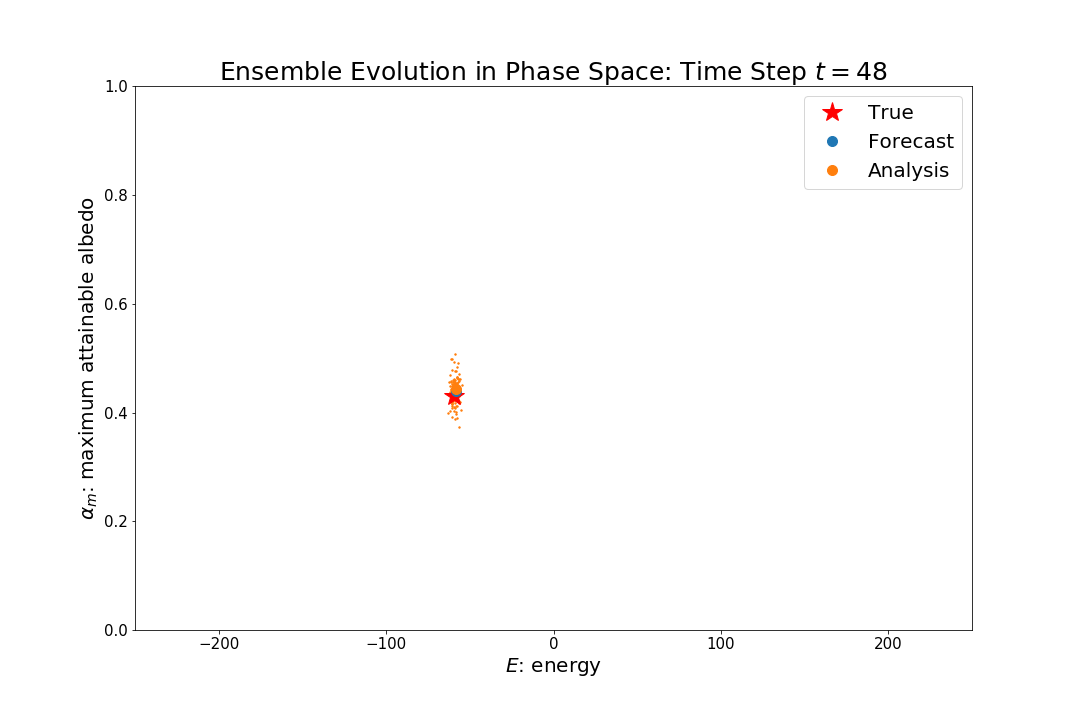
\includegraphics[width=\linewidth]{Figures/EnsembleEvolution_analysis_t=48.png}
\end{frame}
\begin{frame}
\frametitle{Results: Realistic Model}
\centering
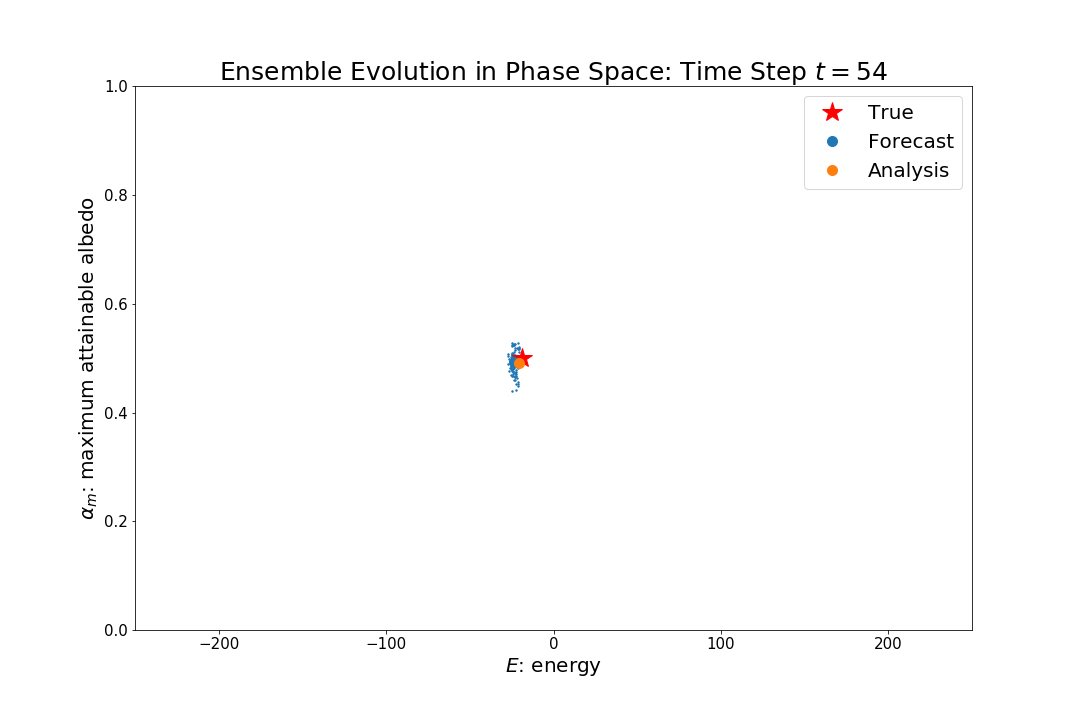
\includegraphics[width=\linewidth]{Figures/EnsembleEvolution_forecast_t=54.png}
\end{frame}
\begin{frame}
\frametitle{Results: Realistic Model}
\centering
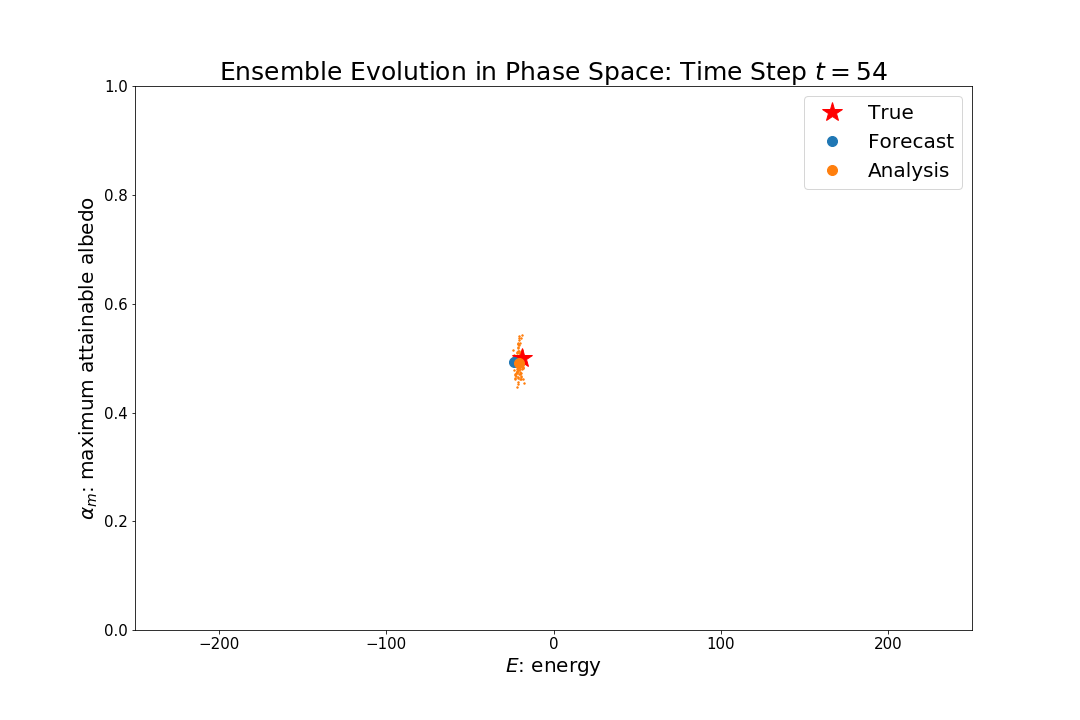
\includegraphics[width=\linewidth]{Figures/EnsembleEvolution_analysis_t=54.png}
\end{frame}
\begin{frame}
\frametitle{Results: Realistic Model}
\centering
\includegraphics[width=\linewidth]{Figures/EnsembleEvolution_forecast_t=60.png}
\end{frame}
\begin{frame}
\frametitle{Results: Realistic Model}
\centering
\includegraphics[width=\linewidth]{Figures/EnsembleEvolution_analysis_t=60.png}
\end{frame}

\begin{frame}
\frametitle{Results: Sparse Data}
{\setlength{\baselineskip}{0.001em}
\tiny{Keep $5\%$ data in $E\in[-50,50]$ for training:}
\begin{center}
\includegraphics[width=0.85\linewidth]{Figures/H_sparse_new.png} 
\end{center}
\tiny{Keep $30\%$ data in $E\in[-50,50]$ for training:}
\begin{center}
\includegraphics[width=0.85\linewidth]{Figures/H_sparse_05_new.png} 
\end{center}
}
\end{frame}

\begin{frame}
\frametitle{Review and Comparison}
\begin{itemize}
\item The figure below compares the performance of different observation operators in terms of forecast and analysis absolute error at each time step.
\item Obviously, data assimilation with the retrieved concentration performs far worse than the others.
\end{itemize} 
\begin{columns}
\begin{column}{0.5\linewidth}
\centering
\includegraphics[width=\linewidth]{Figures/AbsoluteError_E.png}
\end{column}
\begin{column}{0.5\linewidth}
\centering
\includegraphics[width=\linewidth]{Figures/AbsoluteError_am.png}
\end{column}
\end{columns}
\end{frame}

\begin{frame}
\frametitle{Review and Comparison}
\begin{itemize}
	\item The behavior in $E$ and $\alpha_m$ are consistent.
	\item Around the first 30 time steps, $\cH_{\text{ML}}$ does not perform very well. This is expected since, initially, the system is in transient states where the machine learning algorithm does not have sufficient data to learn the true observation operator.
	\item After a while, the error of $\cH_{\text{ML}}$ decreases to roughly the same as $\cH$ and $\cH_{\text{grid}}$.
\end{itemize}
\begin{columns}
\begin{column}{0.5\linewidth}
\centering
\includegraphics[width=\linewidth]{Figures/AbsoluteError_E_2.png}
\end{column}
\begin{column}{0.5\linewidth}
\centering
\includegraphics[width=\linewidth]{Figures/AbsoluteError_am_2.png}
\end{column}
\end{columns}
\end{frame}

\begin{frame}
\frametitle{Discussion}
The experiments demonstrate that
\begin{enumerate}
	\item Assimilating directly on satellite radiance with machine learning observation operator works well and far outperforms assimilating on inaccurately retrieved sea ice concentration. With sufficient amount of data, it is able to achieve roughly the same performance as the true observation operator.
	\item Data density is an important issue. In transient states, without sufficient data, the machine learning observation operator could make large error. However, the performance is still better than assimilating with wrong concentration.
	\item We can use the performance on test set to estimate the error covariance matrix of machine learning observation operator and apply covariance inflation accordingly at corresponding locations in the phase space.
\end{enumerate}
\end{frame}

\begin{frame}
\frametitle{Thank you!}

\begin{itemize}
\item This study is conducted in collaboration with Dr. Christian Sampson under the supervision of Prof. Christopher Jones.
\item All images are from internet.
\end{itemize}

\begin{figure}
\centering
\includegraphics[width=0.6\linewidth]{oldwell_cmyk}
\end{figure}
\end{frame}
%

\end{document}
